\documentclass[12pt,a4paper,oneside]{book}


\usepackage{setspace}
\onehalfspacing

\makeindex
\usepackage{mathtools}
\usepackage{textcomp}
\usepackage{float}
\usepackage{fancyhdr}
\usepackage{makeidx}
\pagestyle{myheadings}
\fancyhf{}
\rhead[\leftmark]{thepage}
\usepackage[toc,page]{appendix}

\usepackage[T1]{fontenc}
\usepackage[utf8]{inputenc}
\usepackage{url}
\setlength {\marginparwidth}{2cm}
\usepackage{todonotes}

\usepackage[all]{xy}
\usepackage{graphicx}
\usepackage{units}
\usepackage{enumerate}
\usepackage[hidelinks]{hyperref}
\usepackage[]{algorithm2e} %algorithm


\usepackage{amssymb, amsmath, amsthm, pict2e}
 \pagestyle{myheadings}

\usepackage{pdfsync}
\usepackage{rotating}
\usepackage{multirow}
\usepackage[normalem]{ulem}
\usepackage{cancel}

\usepackage{color}
%\usepackage[usenames,dvipsnames,svgnames,table]{xcolor}
\usepackage{pgf,tikz}
\usetikzlibrary{decorations,arrows, hobby, graphs, quotes}
\usetikzlibrary{shapes.misc, positioning}
%\usetikzlibrary{decorations.pathmorphing}
\usepgflibrary{decorations.pathreplacing}

\def\arr{\hbox{𝓇}}

\usepackage{environ}
\makeatletter
\newsavebox{\measure@tikzpicture}
\NewEnviron{scaletikzpicturetowidth}[1]{%
  \def\tikz@width{#1}%
  \def\tikzscale{1}\begin{lrbox}{\measure@tikzpicture}%
  \BODY
  \end{lrbox}%
  \pgfmathparse{#1/\wd\measure@tikzpicture}%
  \edef\tikzscale{\pgfmathresult}%
  \BODY
}

%%%%%%%%%%%%%%%%  start macros  %%%%%%%%%%%%%%%%%%%%%%%%%%%%%%%%%
\let\emph\relax % there's no \RedeclareTextFontCommand
\DeclareTextFontCommand{\emph}{\bfseries\em}

\newtheorem{theorem}{Theorem}
\theoremstyle{definition}
\newtheorem{defn}[theorem]{Definition}
\newtheorem{example}[theorem]{Example}
\theoremstyle{remark}
\newtheorem{remark}[theorem]{Remark}
\newtheorem{question}[theorem]{Question}

\theoremstyle{plain}
\newtheorem{lemma}[theorem]{Lemma}
\newtheorem{claim}[theorem]{Claim}
\newtheorem{obs}[theorem]{Observation}
\newtheorem{prop}[theorem]{Proposition}
\newtheorem{corollary}[theorem]{Corollary}
\newtheorem{conjecture}[theorem]{Conjecture}

\newtheorem{hyp}[theorem]{Hypothesis}
\newtheorem{alg}[theorem]{Algorithm}
\numberwithin{theorem}{section}
\newcommand{\powerset}{\raisebox{.15\baselineskip}{\Large\ensuremath{\wp}}}

%\newcommand{\qed}{\mbox{$\Box$}}
%\newcommand{\proof}{\medbreak\par\noindent{\bf Proof. }}
\newtheorem{proofpart}{Part}
\makeatletter
\@addtoreset{proofpart}{theorem}
\makeatother
 \newcommand{\GP}{{\vec{G}}_P}
\newcommand{\GN}{{\vec{G}}_N}

\newcommand{\cover}{\mathrel{\rlap{$\prec$}
                                \rlap{\hskip 0.7em $\cdot$}
                                 \phantom{\prec}}}

\newcommand{\re}{re}

\newcommand{\up}{\mbox{\rm{up}}}
\newcommand{\side}{\mbox{\rm{side}}}
\newcommand{\type}{\mbox{\rm{type}}}


\def\reals{{\mathbb R}}


\newcommand{\ahat}{{\hat{a}}}
\newcommand{\bhat}{{\hat{b}}}
\newcommand{\chat}{{\hat{c}}}
\newcommand{\dhat}{{\hat{d}}}
\newcommand{\bolda}{{\bf{a}}}
\newcommand{\boldb}{{\bf{b}}}
\newcommand{\boldc}{{\bf{c}}}
\newcommand{\boldd}{{\bf{d}}}

\newcommand{\iplus}{{\cal I}^+}
\newcommand{\iminus}{{\cal I}^-}
\newcommand{\ipm}{{\cal I}^{\pm}}
\newcommand{\ipmix}{{\cal I}^{{\cal M}}}

\newcommand{\upl}{{\cal U}^+}
\newcommand{\uminus}{{\cal U}^-}
\newcommand{\upm}{{\cal U}^{\pm}}
\newcommand{\upmix}{{\cal U}^{{\cal M}}}


\newcommand{\ppl}{{\cal P}^+}
\newcommand{\pminus}{{\cal P}^-}
\newcommand{\ppm}{{\cal P}^{\pm}}
\newcommand{\ppmix}{{\cal P}^{{\cal M}}}
\newcommand{\bpm}{{\cal B}^{\pm}}
\newcommand{\tpm}{{\cal T}^{\pm}}
\newcommand{\bpmix}{{\cal B}^{{\cal M}}}
\newcommand{\tpmix}{{\cal T}^{{\cal M}}}

%quoting

\definecolor{quotemark}{gray}{0.7}
\makeatletter
\newlength\origparskip

\newcommand{\fquote}{%
  \@ifnextchar[{\fquote@i}{\fquote@i[]}%]
}

\def\fquote@i[#1]{%
  \def\tempa{#1}%
  \@ifnextchar[{\fquote@ii}{\fquote@ii[]}%]
}%

\def\fquote@ii[#1]{%
  \def\tempb{#1}%
  %\vspace{1em}%
  \noindent%
  \begin{list}{}{%
    \setlength{\leftmargin}{0.3\textwidth}%
    \setlength{\rightmargin}{0.1\textwidth}%
    \setlength{\origparskip}{\parskip}%
  }%
    \item[]%
      \begin{picture}(0,0)%
        \put(-15,-8){\makebox(0,0){\scalebox{4}{%
          \textcolor{quotemark}{\textquotedblright}}}}%
      \end{picture}%
      \begingroup
      \itshape
      \ignorespaces}%

\def\endfquote{%
  \endgroup
  \par
  \raggedleft
  \ifx\tempa\empty
  \else
    {\bfseries --- \tempa\par}%
    \setlength{\parskip}{\origparskip}%
    \ifx\tempb\empty
    \else
      (\tempb)%
  \fi
  \par
  %\vspace{0.5em}%
  \end{list}}
\makeatother

\DeclarePairedDelimiter\ceil{\lceil}{\rceil}
\DeclarePairedDelimiter\floor{\lfloor}{\rfloor}

%%%%%%%%%%%%%%%%  end macros  %%%%%%%%%%%%%%%%%%%%%%%%%%%%%%%%%


\parindent1em
%\parskip1.0ex

\begin{document}

\frontmatter
\begin{titlepage}
\begin{center}
\textbf{UNIVERSIT\'E LIBRE DE BRUXELLES}\\
\textbf{Facult\'e des Sciences}\\
\textbf{D\'epartement d'Informatique}
\vfill{}\vfill{}

{\Huge  Characterization and complexity of \vspace*{.5cm} \linebreak[4] Thin Strip Graphs}

% s \vspace*{.5cm}  \linebreak[4] possibly on many lines   \linebreak[4]  nevertheless a short title is better

{\Huge \par}
\begin{center}{\LARGE Abdeselam El-Haman Abdeselam}\end{center}{\Huge \par}
\vfill{}\vfill{}
\begin{flushright}{\large \textbf{Promotor :} Prof. Jean Cardinal}\\\hfill{}{\large Master Thesis in Computer Sciences}\\
{\large }\hfill{}{}\end{flushright}{\large\par}
\vfill{}\vfill{}\enlargethispage{3cm}
\textbf{Academic year 2018~-~2019}
\end{center}
\end{titlepage}
\newpage
\thispagestyle{empty}
\null

\newenvironment{vcenterpage}
{\newpage\thispagestyle{empty}
\vspace*{\fill}}
{\vspace*{\fill}\par\pagebreak}

\newpage
\thispagestyle{empty}
\vspace*{5cm}

\begin{fquote}[Cave Johnson][Portal 2]
  Science isn't about why -- it's about \emph{why not}.
\end{fquote}


\chapter*{Acknowledgment}
\thispagestyle{empty}

\noindent First of all, I would like to thank my thesis supervisor, Prof. Jean Cardinal for allowing me to be creative and by encouraging me to explore new areas of combinatorics. His courses on complexity and data structures showed me a new facet of computer science I fell in love with. I am also very grateful to him for showing me how to work rigorously during my thesis and also for encouraging me to continue my career in research.

I would also like to thank M. (now Dr.) Keno Merckx for all the help he has given me during the thesis. Keno has shared with me a lot of knowledge that has been useful for me. I will keep his advices preciously.

I also want to thank M. Gilles Geeraerts for all the projects that we shared together in the University. He is the first teacher I had at the University and since, he has been very helpful and open for every question I had. His contagious passion of teaching and pedagogy has pushed me forward to the same direction.

I thanks also the Algorithms group of ULB. Their courses and seminars have been precious for me, and their members have always been open to answer any question, either it was scientific or about my career.

I thank my partner, who has supported me through this whole period and encouraged me to never stop. I also thank my mother for not giving up on me when it wasn't that easy.

Last, but not least, I thank every classmate, colleague, teacher, first-year students, and every person I did not mention for giving me a great experience at the university that I will never forget.\\

Gracias, mamá.

\thispagestyle{empty}
\setcounter{page}{0}
\tableofcontents
\mainmatter
\setcounter{page}{1}

%% CHAPTERS %%
\chapter{Background}
\label{chap:background}

In this chapter we review some definitions and notations of the background knowledge of this thesis. We limit ourselves to the basic notations used during the work. Nevertheless, the bibliography of each subject will be referenced for further details about the topic.

%\todo{Text about background intro}

%%% This is an example first chapter.  You should put chapter/appendix that you
%% write into a separate file, and add a line \include{yourfilename} to
%% main.tex, where `yourfilename.tex' is the name of the chapter/appendix file.
%% You can process specific files by typing their names in at the
%% \files=
%% prompt when you run the file main.tex through LaTeX.
\section{Graphs and intersections}
\label{sec:graphs}


\subsection{Graphs}

A graph $G$ is defined as $G = (V,E)$, where $V$ is the set of vertices and $E$ the set of
edges, where $E \subseteq \binom{V}{2}$. The vertices $v,w \in V$ such that $e = vw \in E$
links are called the \textit{endpoints} of $e$.

\begin{defn}
  An embedding of a graph $G$ into a surface $\Sigma$ is a mapping of $G$ in
  $\Sigma$ where the vertices correspond to distinct points and the edges
  correspond to simple arcs connecting the images of their endpoints.
  \cite{goyalGraphEmbeddingTechniques2017}.
\end{defn}

A graph $G$ is planar if there is an embedding of this graph that does not have
any crossing between the edges.

\begin{defn}
  Let $G = (V,E)$ and $S \subset V$, an induced subgraph is a graph $H$ of $G$ whose
  vertex set is $S$ and its edge set $F = \{vw : v,w \in S, vw \in E\}$.
\end{defn}

\begin{defn}
  Let $G = (V,E)$ its complement graph $\overline{G}$ is the graph such that its edge set
  is defined as: $\{vw: v,w\in V, vw\notin E\}$.
\end{defn}

\begin{defn}
  $H$ is called a \textit{minor} of $G$ if $H$ can be constructed by deleting edges and vertices,
  or contracting edges.
\end{defn}

\begin{theorem}[Kuratowski]
  \label{theo:kura}
  A graph $G$ is planar if and only if it does not contain $K_5$ or $K_{3,3}$ as a minor or
  a induced subgraph.
\end{theorem}

\begin{defn}
  A path $P_n$ in a graph $G$ is a sequence of vertices $v_1v_2v_3\dots v_n$ such
  that $v_iv_{i+1} \in E$.
\end{defn}

\begin{defn}
  A cycle $C_n$ in a graph $G = (V,E)$ is a path $v_1\dots v_n$ such that $v_1 = v_n$.
\end{defn}

\begin{defn}
  A chord of a cycle $C_n$ with $n \geq 4 $ is an edge that connects two non consecutive vertices
  of $C_n$.
\end{defn}

\begin{defn}
  A triangular chord of a cycle is a chord that will create a new triangle ($C_3$).
\end{defn}


\begin{defn}
  A graph $G = (V,E)$ is complete if every pair of distinct $v_1,v_2 \in V$ are
  adjacent. This is denoted $K_n$ with $n$ the size of the graph. If $G$ is an
  induced graph of $H$ then $G$ is a clique of $H$.
\end{defn}

\begin{defn}
  A graph $G$ is bipartite if there exist two disjoint subsets $A,B \subset V$ such
  that $A\cup B = V$ and each edge $e\in E$ has an endpoint on $A$ and the
  another on $B$.
\end{defn}

\begin{defn}
  A bipartite graph $G$ with bipartitions $A$ and $B$ is complete bipartite if
  every pair of vertices $v\in A, w\in B$ are adjacent. It is denoted as $K_{n,m}$,
  being $n$ and $m$ the size of each bipartition.
\end{defn}

Some graphs can be characterized with properties. A property of a graph is a property that
is preserved under all its isomophisms. These properties are called \textit{hereditary} if they
are also preserved under all its induced subgraphs; they are called \textit{minor-hereditary} if they are
also preserved under its minors (e.g. Kuratowski's planar graph characterization [\ref{theo:kura}]).

\begin{defn}
  An forbidden induced subgraph (minor) of a graph class $X$ is a graph such that if it is the induced
  subgraph (minor) of a graph $G$, we know that $G \notin X$.
\end{defn}

The coloration of a graph is a color assignment to each vertex such that the color
of the two endpoints of every edge of the graph is different.

\begin{defn}
  The chromatic number of a graph $\chi(G)$ is the smallest number of colors needed to
  have an acceptable coloration of $G$.
\end{defn}

\begin{defn}
  The clique number of a graph $\omega(G)$ is the size of the biggest clique of $G$. We
  can observe that for every graph: $\chi(G) \geq \omega(G)$.
\end{defn}

\begin{defn}
  A perfect graph is a graph that respects this condition for every induced subgraph:
  $$ \omega(G) = \chi(G)$$
\end{defn}

\begin{theorem}[Lovasz]
  $G$ is perfect if and only if $\overline{G}$ is perfect.
\end{theorem}

\subsection{Intersection graphs}

\begin{defn}
The \textit{intersection graph} of a collection $\zeta$ of objects is the graph
$(\zeta,E)$ such that $c_1c_2\in E \Leftrightarrow c_1 \cap c_2 \neq \varnothing$.
\end{defn}

An intersection can be seen as a relationship between two objects. In this thesis, it will be important to define these relations more formally to characterize intersection graphs.

\begin{defn}
  A partial order is a binary relation $\leq$ over a set $A$ satisfying these axioms:
  \begin{itemize}
    \item if $a \leq b$ and $b \leq a$ then $a = b$ (antisymmetry).
    \item if $a \leq b$ and $b \leq c$ then $a \leq c$ (transitivity).
    \item $a \leq a$ (reflexivity).
  \end{itemize}
\end{defn}

\begin{defn}
  A total order is a partial order where the reflexivity order is replaced by the connex property:
  $$a \leq b\ \text{or}\  b \leq a$$
\end{defn}

\begin{defn}
   A partially ordered set or poset  $(S,\leq)$ where $S$ a set and $\leq$ a partial
   order on $S$.
\end{defn}

\begin{defn}
  A spanning order $(V,<)$ of a graph $G = (V,E)$ is a total order on $V$ such that for any three vertices $u < v < w$:

  $$uw \in E \to uv \in E\ \text{or}\ vw \in E$$
\end{defn}


\begin{defn}
  A graph $G = (V,E)$ is a comparibility graph if there exists a partial order
  $\leq$ such that $vw \in E \Leftrightarrow v \leq w$ or $w \leq v$.
  Equivalently, $G$ is a comparability graph if it is the comparability graph of
  a poset. For example, the Hasse diagram (figure \ref{fig:hasse}) is a
  comparability graph where the relation is inclusion.
\end{defn}

\begin{defn}
  A graph $G = (V,E)$ is a co-comparability graph if its complement is a comparability graph.
\end{defn}

There are multiple characterizations for the co-comparability graph class; we will see one that uses a poset to characterize it:

\begin{theorem}[Damaschke \cite{damaschkeDistancesCocomparabilityGraphs1992}]
  \label{theo:spanning}
  A graph $G$ is a co-comparability graph if and only if it has a spanning order.
\end{theorem}


\begin{figure}
\centering

\begin{scaletikzpicturetowidth}{\textwidth}
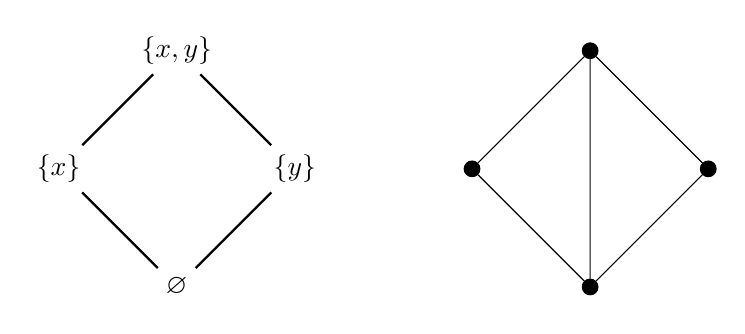
\begin{tikzpicture}[scale=1.5]

  % poset
  \draw (-1cm,0cm) node (v2) {$\{x\}$};
  \draw (1cm,0cm)  node (v3) { $\{y\}$ };
  \draw (0cm,-1cm) node (v4) {$\varnothing$};
  \draw (0cm,1cm)  node (v1) {$\{x,y\}$};

  \draw[thick]  (v1) edge (v2);
  \draw[thick]  (v3) edge (v1);
  \draw[thick]  (v3) edge (v4);
  \draw[thick]  (v2) edge (v4);

  % graph
  \node[draw,circle,inner sep=2pt,fill,label distance=1cm] (v1g) at (3.5,1) {};
  \node[draw,circle,inner sep=2pt,fill,label distance=1cm] (v2g) at (3.5,-1) {};
  \node[draw,circle,inner sep=2pt,fill,label distance=1cm] (v3g) at (4.5,0) {};
  \node[draw,circle,inner sep=2pt,fill,label distance=1cm] (v4g) at (2.5,0) {};
  \draw  (v1g) edge (v2g);
  \draw  (v1g) edge (v4g);
  \draw  (v4g) edge (v2g);
  \draw  (v1g) edge (v3g);
  \draw  (v3g) edge (v2g);

\end{tikzpicture}
\end{scaletikzpicturetowidth}

\caption{On the left, Hasse diagram of a poset of the power set of 2 elements ordered by inclusion.
On the right, the comparability graph of this poset.}
\label{fig:hasse}
\end{figure}

\subsubsection{Disks}

A disk graph $G$ is a graph that is an intersection graph of disks on the plane, when the size
of the disk is unitary, we talk about unit disk graphs. This class of graphs
is important for this thesis, as thin strip graphs are a sub-class of
unit disk graphs.

We will refer to the unit disk graph class as UDG and an example of a realization
can be found in the figure \ref{fig:udg}.

\paragraph{Induced forbidden subgraphs} The characterization of this class with respect to
its induced forbidden subgraphs has been studied \cite{atminasForbiddenInducedSubgraphs2016}.

\begin{theorem}[Atminas-Zamaraev]
  For every integer $k > 1$, $\overline{K_2 + C_{2k+1}}$ is a minimal induced subgraph of UDG.
\end{theorem}

\begin{theorem}[Atminas-Zamaraev]
  For every integer $k > 4$, $\overline{C_{2k}}$ is a minimal induced subgraph of UDG.
\end{theorem}

\begin{figure}
\centering

\begin{scaletikzpicturetowidth}{\textwidth}
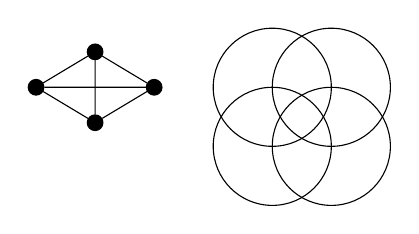
\begin{tikzpicture}[scale=1.5]

  \draw (-0.5,2.5) circle [radius=0.5];
  \draw (0,2.5) circle [radius=0.5];
  \draw (-0.5,2) circle [radius=0.5];
  \draw (0,2) circle [radius=0.5];


  \node[draw,circle,inner sep=2pt,fill,label distance=1cm] (v1) at (-2.5,2.5) {};

  \node[draw,circle,inner sep=2pt,fill,label distance=1cm] (v2) at (-2,2.2) {};
  \node[draw,circle,inner sep=2pt,fill,label distance=1cm] (v3) at (-2,2.8) {};
  \node[draw,circle,inner sep=2pt,fill,label distance=1cm] (v4) at (-1.5,2.5) {};

  \draw  (v3) edge (v2);
  \draw  (v4) edge (v1);
  \draw  (v3) edge (v1);
  \draw  (v4) edge (v2);
  \draw  (v3) edge (v4);
  \draw  (v1) edge (v2);

\end{tikzpicture}
\end{scaletikzpicturetowidth}

\caption{Realization of a UDG (Unit Disk Graph).}
\label{fig:udg}
\end{figure}

%\input{chap1/complexity}
%%% This is an example first chapter.  You should put chapter/appendix that you
%% write into a separate file, and add a line \include{yourfilename} to
%% main.tex, where `yourfilename.tex' is the name of the chapter/appendix file.
%% You can process specific files by typing their names in at the
%% \files=
%% prompt when you run the file main.tex through LaTeX.
\section{Geometry}
\label{sec:geom}

\begin{defn}
  $\text{dist}(a,b)$ denotes the distance between the points $a$ and $b$ and is calculated with:

  $$\text{dist}(a,b) = \sqrt{(a_x - b_x)^2 + (a_y - b_y)^2}$$
\end{defn}

The intersection of convex objects is a matter well studied for multiple
subjects. In our case, it is interesting to know some properties about
the intersection of disks, those ones being convex objects.

A set $S$ is convex if:
$$\forall p,q \in S\  \forall \lambda \in [0,1]: (1-\lambda)p + \lambda q \in S$$

\subsection{Stabbing}
A \textit{stabbing} is a point that traverses a set of intersecting objects. A lot of
research has been done \cite{schlipf2013stabbing} on the minimal amount of stabbings to
cover every object in a set. Stabbings can also be done with more complex structures
than points, in that case we are talking about \textit{coverings}.

\begin{theorem}[Helly]
  Given a set $Q$ of objects in $\mathbb{R}^d$, if for each subset of $Q$ of
  size $d+1$ their intersection is non empty, then $\bigcap_{q \in Q} \neq
  \varnothing$. \cite{Helly1923175}
\end{theorem}

\begin{theorem}
  The problem that for a set of $n$ disks whether there exists a regular n-gon
  whose vertices stab every disk of the set can be decided in $O(n^{10.5} / \sqrt{\log(n)})$ \cite{schlipf2013stabbing}
\end{theorem}

\subsection{Coin graphs}

Penny graphs can be defined as disk graphs where the disks can just touch each
other without overlapping. A famous theorem is derived from this class of graphs:
the circle packing theorem.

\begin{theorem}[Circle packing theorem]
  The circle packing theorem states that every simple connected planar graph
  $G$ is a penny graph. \cite{doi:10.1137/0406017}
\end{theorem}

\begin{corollary}
  Planar graphs $\subseteq$ disk graphs \cite{spinradEfficientGraphRepresentations2012}.
\end{corollary}

\begin{figure}
\centering
\includegraphics[width=1.0\textwidth]{res/circle_packing}
\caption{Circle packing of a planar graph. \cite{nachmiasPlanarMapsRandom2016}}
\label{fig:circle}
\end{figure}


\section{Graph theory}

A \emph{graph} is defined as a tuple $G = (V,E)$ where $V$ is the set of \emph{vertices} and $E$. When the the set of \emph{edges}, where $E = \binom{V}{2}$. If two vertices are share the same edge $e$ they are called \emph{adjacent} and also the \emph{endpoints} of $e$. A \emph{subgraph} $H = (V', E')$ of a graph $G$ is a graph such that $V' \subseteq V$ and $E' \subseteq E$. An \emph{induced subgraph} of a graph is a subgraph $H$ of a graph $G$ such that for every edge of $G$ is also in $H$ if its two endpoints are in $V'$. A \emph{clique} is a subgraph such that every vertex is adjacent to each other. A graph that is also a clique is called a \emph{complete graph} and it is denoted as $K_n$. A graph is \emph{bipartite} if there exist two disjoint subsets of the vertex set $A \cup B = V$ such that two vertices of the same subset are not adjacent. A \emph{complete bipartite graph} $K_{n,m}$ is a bipartite graph such that $v \in A$ and $w \in B$ implies $vw \in E$ where $n$ and $m$ are the size of each bipartition.

A \emph{path} $P_n = v_1\dots v_{n+1}$ of a graph is a sequence of $n$ vertices such that two consequent vertices are adjacent. A \emph{cycle} is a path $C_n = v_1\dots v_nv_{n+1}$ such that $v_1=v_{n+1}$. A graph is \emph{connected} if there exists a path between every pair of vertices. A \emph{chord} of a cycle $C_n$ with $n \geqslant 4$ is an edge that connects two non adjacent vertices of the cycle. A graph is \emph{chordal} if there is a chord in every cycle bigger than four.

\subsection{Intersection graphs}

\begin{figure}
\centering

\begin{scaletikzpicturetowidth}{\textwidth}
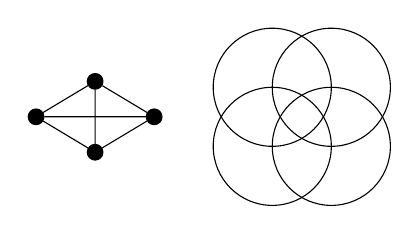
\begin{tikzpicture}[scale=1.5]

  \draw (-0.5,2.5) circle [radius=0.5];
  \draw (0,2.5) circle [radius=0.5];
  \draw (-0.5,2) circle [radius=0.5];
  \draw (0,2) circle [radius=0.5];


  \node[draw,circle,inner sep=2pt,fill,label distance=1cm] (v1) at (-2.5,2.25) {};

  \node[draw,circle,inner sep=2pt,fill,label distance=1cm] (v2) at (-2,1.95) {};
  \node[draw,circle,inner sep=2pt,fill,label distance=1cm] (v3) at (-2,2.55) {};
  \node[draw,circle,inner sep=2pt,fill,label distance=1cm] (v4) at (-1.5,2.25) {};

  \draw  (v3) edge (v2);
  \draw  (v4) edge (v1);
  \draw  (v3) edge (v1);
  \draw  (v4) edge (v2);
  \draw  (v3) edge (v4);
  \draw  (v1) edge (v2);

\end{tikzpicture}
\end{scaletikzpicturetowidth}

\caption{Realization of a UDG (unit disk graph).}
\label{fig:udg}
\end{figure}


An \emph{intersection graph} is a graph $G = (\zeta,E)$ of a collection of objects $\zeta$ is a graph such that $v,w \in \zeta$ and $v \cup w \neq \varnothing$ implies that $vw \in E$. An \emph{interval graph} is an intersection graph of intervals on the plane; when the size of the intervals is equal they are called \emph{unit interval graphs}. A \emph{unit disk graph} is an intersection graph of disks on a plane that have the same diameter - you can find an example in Figure \ref{fig:udg}.

\section{Order and set theory}

The \emph{powerset} $\powerset(S)$ of a set $S$ is the set of subsets of $S$. A \emph{partial order} is a binary relation $\leqslant$ over a set $A$ satisfying three axioms:

\begin{itemize}
  \item if $a \leqslant b$ and $b \leqslant a$ then $a = b$ (\emph{antisymmetry}).
  \item if $a \leqslant b$ and $b \leqslant c$ then $a \leqslant c$ (\emph{transitivity}).
  \item $a \leqslant a$ (\emph{reflexivity}).
\end{itemize}

\begin{figure}
\centering

\begin{scaletikzpicturetowidth}{\textwidth}
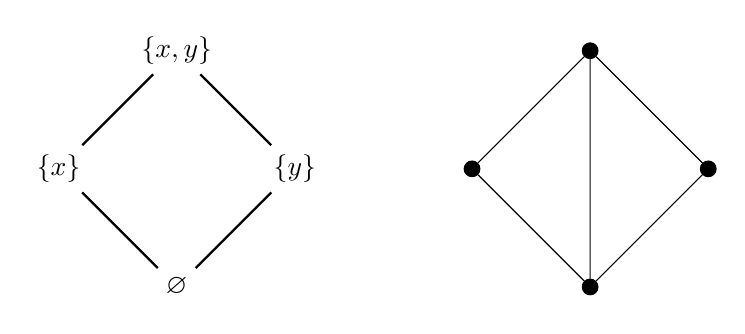
\begin{tikzpicture}[scale=1.5]

  % poset
  \draw (-1cm,0cm) node (v2) {$\{x\}$};
  \draw (1cm,0cm)  node (v3) { $\{y\}$ };
  \draw (0cm,-1cm) node (v4) {$\varnothing$};
  \draw (0cm,1cm)  node (v1) {$\{x,y\}$};

  \draw[thick]  (v1) edge (v2);
  \draw[thick]  (v3) edge (v1);
  \draw[thick]  (v3) edge (v4);
  \draw[thick]  (v2) edge (v4);

  % graph
  \node[draw,circle,inner sep=2pt,fill,label distance=1cm] (v1g) at (3.5,1) {};
  \node[draw,circle,inner sep=2pt,fill,label distance=1cm] (v2g) at (3.5,-1) {};
  \node[draw,circle,inner sep=2pt,fill,label distance=1cm] (v3g) at (4.5,0) {};
  \node[draw,circle,inner sep=2pt,fill,label distance=1cm] (v4g) at (2.5,0) {};
  \draw  (v1g) edge (v2g);
  \draw  (v1g) edge (v4g);
  \draw  (v4g) edge (v2g);
  \draw  (v1g) edge (v3g);
  \draw  (v3g) edge (v2g);

\end{tikzpicture}
\end{scaletikzpicturetowidth}

\caption{On the left, Hasse diagram of a poset of the power set of 2 elements ordered by inclusion.
On the right, the comparability graph of this poset.}
\label{fig:hasse}
\end{figure}

In the other side, a \emph{total order} is a partial order where the reflexivity order is replaced by the \emph{connexity} property -- $a \leq b\ \text{or}\  b \leq a$. A \emph{partially ordered set} (or \emph{poset}) $(S,\leqslant)$ is a set such that the elements of $S$ are partially ordered by the relation $\leqslant$. A good way to represent a poset is the \emph{Hasse diagram} (figure \ref{fig:hasse}).

\subsection{Comparability graphs}

A \emph{spanning order} $(V,<)$ on a graph $G = (V,E)$ is a total order on $V$ such that for any three vertices $u < v < w$:

  $$uw \in E \to uv \in E\ \text{or}\ vw \in E$$

The class of comparability graphs are built on the ideas of order theory. A graph $G$ is a \emph{comparability graph} if there exists a partial order $\leqslant$ such that $uv \in E \Leftrightarrow v \leqslant w\  \text{or}\  w \leqslant v$.

\section{Geometry}

\chapter{Background}
\label{chap:background}

In this chapter we review some definitions and notations of the background knowledge of this thesis. We limit ourselves to the basic notations used during the work. Nevertheless, the bibliography of each subject will be referenced for further details about the topic.

%\todo{Text about background intro}

%%% This is an example first chapter.  You should put chapter/appendix that you
%% write into a separate file, and add a line \include{yourfilename} to
%% main.tex, where `yourfilename.tex' is the name of the chapter/appendix file.
%% You can process specific files by typing their names in at the
%% \files=
%% prompt when you run the file main.tex through LaTeX.
\section{Graphs and intersections}
\label{sec:graphs}


\subsection{Graphs}

A graph $G$ is defined as $G = (V,E)$, where $V$ is the set of vertices and $E$ the set of
edges, where $E \subseteq \binom{V}{2}$. The vertices $v,w \in V$ such that $e = vw \in E$
links are called the \textit{endpoints} of $e$.

\begin{defn}
  An embedding of a graph $G$ into a surface $\Sigma$ is a mapping of $G$ in
  $\Sigma$ where the vertices correspond to distinct points and the edges
  correspond to simple arcs connecting the images of their endpoints.
  \cite{goyalGraphEmbeddingTechniques2017}.
\end{defn}

A graph $G$ is planar if there is an embedding of this graph that does not have
any crossing between the edges.

\begin{defn}
  Let $G = (V,E)$ and $S \subset V$, an induced subgraph is a graph $H$ of $G$ whose
  vertex set is $S$ and its edge set $F = \{vw : v,w \in S, vw \in E\}$.
\end{defn}

\begin{defn}
  Let $G = (V,E)$ its complement graph $\overline{G}$ is the graph such that its edge set
  is defined as: $\{vw: v,w\in V, vw\notin E\}$.
\end{defn}

\begin{defn}
  $H$ is called a \textit{minor} of $G$ if $H$ can be constructed by deleting edges and vertices,
  or contracting edges.
\end{defn}

\begin{theorem}[Kuratowski]
  \label{theo:kura}
  A graph $G$ is planar if and only if it does not contain $K_5$ or $K_{3,3}$ as a minor or
  a induced subgraph.
\end{theorem}

\begin{defn}
  A path $P_n$ in a graph $G$ is a sequence of vertices $v_1v_2v_3\dots v_n$ such
  that $v_iv_{i+1} \in E$.
\end{defn}

\begin{defn}
  A cycle $C_n$ in a graph $G = (V,E)$ is a path $v_1\dots v_n$ such that $v_1 = v_n$.
\end{defn}

\begin{defn}
  A chord of a cycle $C_n$ with $n \geq 4 $ is an edge that connects two non consecutive vertices
  of $C_n$.
\end{defn}

\begin{defn}
  A triangular chord of a cycle is a chord that will create a new triangle ($C_3$).
\end{defn}


\begin{defn}
  A graph $G = (V,E)$ is complete if every pair of distinct $v_1,v_2 \in V$ are
  adjacent. This is denoted $K_n$ with $n$ the size of the graph. If $G$ is an
  induced graph of $H$ then $G$ is a clique of $H$.
\end{defn}

\begin{defn}
  A graph $G$ is bipartite if there exist two disjoint subsets $A,B \subset V$ such
  that $A\cup B = V$ and each edge $e\in E$ has an endpoint on $A$ and the
  another on $B$.
\end{defn}

\begin{defn}
  A bipartite graph $G$ with bipartitions $A$ and $B$ is complete bipartite if
  every pair of vertices $v\in A, w\in B$ are adjacent. It is denoted as $K_{n,m}$,
  being $n$ and $m$ the size of each bipartition.
\end{defn}

Some graphs can be characterized with properties. A property of a graph is a property that
is preserved under all its isomophisms. These properties are called \textit{hereditary} if they
are also preserved under all its induced subgraphs; they are called \textit{minor-hereditary} if they are
also preserved under its minors (e.g. Kuratowski's planar graph characterization [\ref{theo:kura}]).

\begin{defn}
  An forbidden induced subgraph (minor) of a graph class $X$ is a graph such that if it is the induced
  subgraph (minor) of a graph $G$, we know that $G \notin X$.
\end{defn}

The coloration of a graph is a color assignment to each vertex such that the color
of the two endpoints of every edge of the graph is different.

\begin{defn}
  The chromatic number of a graph $\chi(G)$ is the smallest number of colors needed to
  have an acceptable coloration of $G$.
\end{defn}

\begin{defn}
  The clique number of a graph $\omega(G)$ is the size of the biggest clique of $G$. We
  can observe that for every graph: $\chi(G) \geq \omega(G)$.
\end{defn}

\begin{defn}
  A perfect graph is a graph that respects this condition for every induced subgraph:
  $$ \omega(G) = \chi(G)$$
\end{defn}

\begin{theorem}[Lovasz]
  $G$ is perfect if and only if $\overline{G}$ is perfect.
\end{theorem}

\subsection{Intersection graphs}

\begin{defn}
The \textit{intersection graph} of a collection $\zeta$ of objects is the graph
$(\zeta,E)$ such that $c_1c_2\in E \Leftrightarrow c_1 \cap c_2 \neq \varnothing$.
\end{defn}

An intersection can be seen as a relationship between two objects. In this thesis, it will be important to define these relations more formally to characterize intersection graphs.

\begin{defn}
  A partial order is a binary relation $\leq$ over a set $A$ satisfying these axioms:
  \begin{itemize}
    \item if $a \leq b$ and $b \leq a$ then $a = b$ (antisymmetry).
    \item if $a \leq b$ and $b \leq c$ then $a \leq c$ (transitivity).
    \item $a \leq a$ (reflexivity).
  \end{itemize}
\end{defn}

\begin{defn}
  A total order is a partial order where the reflexivity order is replaced by the connex property:
  $$a \leq b\ \text{or}\  b \leq a$$
\end{defn}

\begin{defn}
   A partially ordered set or poset  $(S,\leq)$ where $S$ a set and $\leq$ a partial
   order on $S$.
\end{defn}

\begin{defn}
  A spanning order $(V,<)$ of a graph $G = (V,E)$ is a total order on $V$ such that for any three vertices $u < v < w$:

  $$uw \in E \to uv \in E\ \text{or}\ vw \in E$$
\end{defn}


\begin{defn}
  A graph $G = (V,E)$ is a comparibility graph if there exists a partial order
  $\leq$ such that $vw \in E \Leftrightarrow v \leq w$ or $w \leq v$.
  Equivalently, $G$ is a comparability graph if it is the comparability graph of
  a poset. For example, the Hasse diagram (figure \ref{fig:hasse}) is a
  comparability graph where the relation is inclusion.
\end{defn}

\begin{defn}
  A graph $G = (V,E)$ is a co-comparability graph if its complement is a comparability graph.
\end{defn}

There are multiple characterizations for the co-comparability graph class; we will see one that uses a poset to characterize it:

\begin{theorem}[Damaschke \cite{damaschkeDistancesCocomparabilityGraphs1992}]
  \label{theo:spanning}
  A graph $G$ is a co-comparability graph if and only if it has a spanning order.
\end{theorem}


\begin{figure}
\centering

\begin{scaletikzpicturetowidth}{\textwidth}
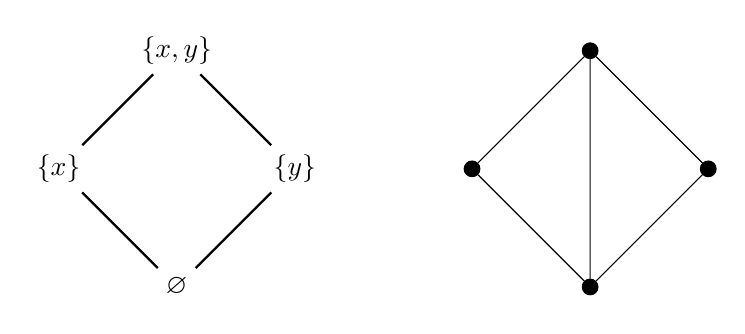
\begin{tikzpicture}[scale=1.5]

  % poset
  \draw (-1cm,0cm) node (v2) {$\{x\}$};
  \draw (1cm,0cm)  node (v3) { $\{y\}$ };
  \draw (0cm,-1cm) node (v4) {$\varnothing$};
  \draw (0cm,1cm)  node (v1) {$\{x,y\}$};

  \draw[thick]  (v1) edge (v2);
  \draw[thick]  (v3) edge (v1);
  \draw[thick]  (v3) edge (v4);
  \draw[thick]  (v2) edge (v4);

  % graph
  \node[draw,circle,inner sep=2pt,fill,label distance=1cm] (v1g) at (3.5,1) {};
  \node[draw,circle,inner sep=2pt,fill,label distance=1cm] (v2g) at (3.5,-1) {};
  \node[draw,circle,inner sep=2pt,fill,label distance=1cm] (v3g) at (4.5,0) {};
  \node[draw,circle,inner sep=2pt,fill,label distance=1cm] (v4g) at (2.5,0) {};
  \draw  (v1g) edge (v2g);
  \draw  (v1g) edge (v4g);
  \draw  (v4g) edge (v2g);
  \draw  (v1g) edge (v3g);
  \draw  (v3g) edge (v2g);

\end{tikzpicture}
\end{scaletikzpicturetowidth}

\caption{On the left, Hasse diagram of a poset of the power set of 2 elements ordered by inclusion.
On the right, the comparability graph of this poset.}
\label{fig:hasse}
\end{figure}

\subsubsection{Disks}

A disk graph $G$ is a graph that is an intersection graph of disks on the plane, when the size
of the disk is unitary, we talk about unit disk graphs. This class of graphs
is important for this thesis, as thin strip graphs are a sub-class of
unit disk graphs.

We will refer to the unit disk graph class as UDG and an example of a realization
can be found in the figure \ref{fig:udg}.

\paragraph{Induced forbidden subgraphs} The characterization of this class with respect to
its induced forbidden subgraphs has been studied \cite{atminasForbiddenInducedSubgraphs2016}.

\begin{theorem}[Atminas-Zamaraev]
  For every integer $k > 1$, $\overline{K_2 + C_{2k+1}}$ is a minimal induced subgraph of UDG.
\end{theorem}

\begin{theorem}[Atminas-Zamaraev]
  For every integer $k > 4$, $\overline{C_{2k}}$ is a minimal induced subgraph of UDG.
\end{theorem}

\begin{figure}
\centering

\begin{scaletikzpicturetowidth}{\textwidth}
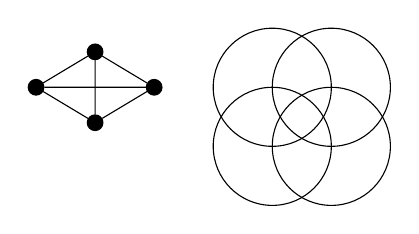
\begin{tikzpicture}[scale=1.5]

  \draw (-0.5,2.5) circle [radius=0.5];
  \draw (0,2.5) circle [radius=0.5];
  \draw (-0.5,2) circle [radius=0.5];
  \draw (0,2) circle [radius=0.5];


  \node[draw,circle,inner sep=2pt,fill,label distance=1cm] (v1) at (-2.5,2.5) {};

  \node[draw,circle,inner sep=2pt,fill,label distance=1cm] (v2) at (-2,2.2) {};
  \node[draw,circle,inner sep=2pt,fill,label distance=1cm] (v3) at (-2,2.8) {};
  \node[draw,circle,inner sep=2pt,fill,label distance=1cm] (v4) at (-1.5,2.5) {};

  \draw  (v3) edge (v2);
  \draw  (v4) edge (v1);
  \draw  (v3) edge (v1);
  \draw  (v4) edge (v2);
  \draw  (v3) edge (v4);
  \draw  (v1) edge (v2);

\end{tikzpicture}
\end{scaletikzpicturetowidth}

\caption{Realization of a UDG (Unit Disk Graph).}
\label{fig:udg}
\end{figure}

%\input{chap1/complexity}
%%% This is an example first chapter.  You should put chapter/appendix that you
%% write into a separate file, and add a line \include{yourfilename} to
%% main.tex, where `yourfilename.tex' is the name of the chapter/appendix file.
%% You can process specific files by typing their names in at the
%% \files=
%% prompt when you run the file main.tex through LaTeX.
\section{Geometry}
\label{sec:geom}

\begin{defn}
  $\text{dist}(a,b)$ denotes the distance between the points $a$ and $b$ and is calculated with:

  $$\text{dist}(a,b) = \sqrt{(a_x - b_x)^2 + (a_y - b_y)^2}$$
\end{defn}

The intersection of convex objects is a matter well studied for multiple
subjects. In our case, it is interesting to know some properties about
the intersection of disks, those ones being convex objects.

A set $S$ is convex if:
$$\forall p,q \in S\  \forall \lambda \in [0,1]: (1-\lambda)p + \lambda q \in S$$

\subsection{Stabbing}
A \textit{stabbing} is a point that traverses a set of intersecting objects. A lot of
research has been done \cite{schlipf2013stabbing} on the minimal amount of stabbings to
cover every object in a set. Stabbings can also be done with more complex structures
than points, in that case we are talking about \textit{coverings}.

\begin{theorem}[Helly]
  Given a set $Q$ of objects in $\mathbb{R}^d$, if for each subset of $Q$ of
  size $d+1$ their intersection is non empty, then $\bigcap_{q \in Q} \neq
  \varnothing$. \cite{Helly1923175}
\end{theorem}

\begin{theorem}
  The problem that for a set of $n$ disks whether there exists a regular n-gon
  whose vertices stab every disk of the set can be decided in $O(n^{10.5} / \sqrt{\log(n)})$ \cite{schlipf2013stabbing}
\end{theorem}

\subsection{Coin graphs}

Penny graphs can be defined as disk graphs where the disks can just touch each
other without overlapping. A famous theorem is derived from this class of graphs:
the circle packing theorem.

\begin{theorem}[Circle packing theorem]
  The circle packing theorem states that every simple connected planar graph
  $G$ is a penny graph. \cite{doi:10.1137/0406017}
\end{theorem}

\begin{corollary}
  Planar graphs $\subseteq$ disk graphs \cite{spinradEfficientGraphRepresentations2012}.
\end{corollary}

\begin{figure}
\centering
\includegraphics[width=1.0\textwidth]{res/circle_packing}
\caption{Circle packing of a planar graph. \cite{nachmiasPlanarMapsRandom2016}}
\label{fig:circle}
\end{figure}


\section{Graph theory}

A \emph{graph} is defined as a tuple $G = (V,E)$ where $V$ is the set of \emph{vertices} and $E$. When the the set of \emph{edges}, where $E = \binom{V}{2}$. If two vertices are share the same edge $e$ they are called \emph{adjacent} and also the \emph{endpoints} of $e$. A \emph{subgraph} $H = (V', E')$ of a graph $G$ is a graph such that $V' \subseteq V$ and $E' \subseteq E$. An \emph{induced subgraph} of a graph is a subgraph $H$ of a graph $G$ such that for every edge of $G$ is also in $H$ if its two endpoints are in $V'$. A \emph{clique} is a subgraph such that every vertex is adjacent to each other. A graph that is also a clique is called a \emph{complete graph} and it is denoted as $K_n$. A graph is \emph{bipartite} if there exist two disjoint subsets of the vertex set $A \cup B = V$ such that two vertices of the same subset are not adjacent. A \emph{complete bipartite graph} $K_{n,m}$ is a bipartite graph such that $v \in A$ and $w \in B$ implies $vw \in E$ where $n$ and $m$ are the size of each bipartition.

A \emph{path} $P_n = v_1\dots v_{n+1}$ of a graph is a sequence of $n$ vertices such that two consequent vertices are adjacent. A \emph{cycle} is a path $C_n = v_1\dots v_nv_{n+1}$ such that $v_1=v_{n+1}$. A graph is \emph{connected} if there exists a path between every pair of vertices. A \emph{chord} of a cycle $C_n$ with $n \geqslant 4$ is an edge that connects two non adjacent vertices of the cycle. A graph is \emph{chordal} if there is a chord in every cycle bigger than four.

\subsection{Intersection graphs}

\begin{figure}
\centering

\begin{scaletikzpicturetowidth}{\textwidth}
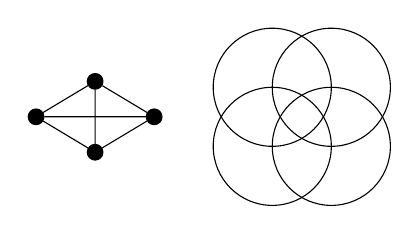
\begin{tikzpicture}[scale=1.5]

  \draw (-0.5,2.5) circle [radius=0.5];
  \draw (0,2.5) circle [radius=0.5];
  \draw (-0.5,2) circle [radius=0.5];
  \draw (0,2) circle [radius=0.5];


  \node[draw,circle,inner sep=2pt,fill,label distance=1cm] (v1) at (-2.5,2.25) {};

  \node[draw,circle,inner sep=2pt,fill,label distance=1cm] (v2) at (-2,1.95) {};
  \node[draw,circle,inner sep=2pt,fill,label distance=1cm] (v3) at (-2,2.55) {};
  \node[draw,circle,inner sep=2pt,fill,label distance=1cm] (v4) at (-1.5,2.25) {};

  \draw  (v3) edge (v2);
  \draw  (v4) edge (v1);
  \draw  (v3) edge (v1);
  \draw  (v4) edge (v2);
  \draw  (v3) edge (v4);
  \draw  (v1) edge (v2);

\end{tikzpicture}
\end{scaletikzpicturetowidth}

\caption{Realization of a UDG (unit disk graph).}
\label{fig:udg}
\end{figure}


An \emph{intersection graph} is a graph $G = (\zeta,E)$ of a collection of objects $\zeta$ is a graph such that $v,w \in \zeta$ and $v \cup w \neq \varnothing$ implies that $vw \in E$. An \emph{interval graph} is an intersection graph of intervals on the plane; when the size of the intervals is equal they are called \emph{unit interval graphs}. A \emph{unit disk graph} is an intersection graph of disks on a plane that have the same diameter - you can find an example in Figure \ref{fig:udg}.

\section{Order and set theory}

The \emph{powerset} $\powerset(S)$ of a set $S$ is the set of subsets of $S$. A \emph{partial order} is a binary relation $\leqslant$ over a set $A$ satisfying three axioms:

\begin{itemize}
  \item if $a \leqslant b$ and $b \leqslant a$ then $a = b$ (\emph{antisymmetry}).
  \item if $a \leqslant b$ and $b \leqslant c$ then $a \leqslant c$ (\emph{transitivity}).
  \item $a \leqslant a$ (\emph{reflexivity}).
\end{itemize}

\begin{figure}
\centering

\begin{scaletikzpicturetowidth}{\textwidth}
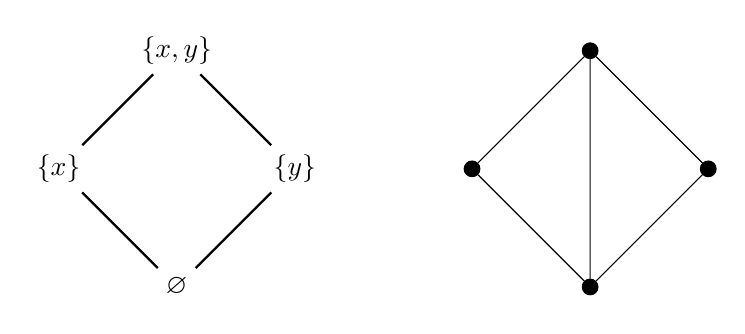
\begin{tikzpicture}[scale=1.5]

  % poset
  \draw (-1cm,0cm) node (v2) {$\{x\}$};
  \draw (1cm,0cm)  node (v3) { $\{y\}$ };
  \draw (0cm,-1cm) node (v4) {$\varnothing$};
  \draw (0cm,1cm)  node (v1) {$\{x,y\}$};

  \draw[thick]  (v1) edge (v2);
  \draw[thick]  (v3) edge (v1);
  \draw[thick]  (v3) edge (v4);
  \draw[thick]  (v2) edge (v4);

  % graph
  \node[draw,circle,inner sep=2pt,fill,label distance=1cm] (v1g) at (3.5,1) {};
  \node[draw,circle,inner sep=2pt,fill,label distance=1cm] (v2g) at (3.5,-1) {};
  \node[draw,circle,inner sep=2pt,fill,label distance=1cm] (v3g) at (4.5,0) {};
  \node[draw,circle,inner sep=2pt,fill,label distance=1cm] (v4g) at (2.5,0) {};
  \draw  (v1g) edge (v2g);
  \draw  (v1g) edge (v4g);
  \draw  (v4g) edge (v2g);
  \draw  (v1g) edge (v3g);
  \draw  (v3g) edge (v2g);

\end{tikzpicture}
\end{scaletikzpicturetowidth}

\caption{On the left, Hasse diagram of a poset of the power set of 2 elements ordered by inclusion.
On the right, the comparability graph of this poset.}
\label{fig:hasse}
\end{figure}

In the other side, a \emph{total order} is a partial order where the reflexivity order is replaced by the \emph{connexity} property -- $a \leq b\ \text{or}\  b \leq a$. A \emph{partially ordered set} (or \emph{poset}) $(S,\leqslant)$ is a set such that the elements of $S$ are partially ordered by the relation $\leqslant$. A good way to represent a poset is the \emph{Hasse diagram} (figure \ref{fig:hasse}).

\subsection{Comparability graphs}

A \emph{spanning order} $(V,<)$ on a graph $G = (V,E)$ is a total order on $V$ such that for any three vertices $u < v < w$:

  $$uw \in E \to uv \in E\ \text{or}\ vw \in E$$

The class of comparability graphs are built on the ideas of order theory. A graph $G$ is a \emph{comparability graph} if there exists a partial order $\leqslant$ such that $uv \in E \Leftrightarrow v \leqslant w\  \text{or}\  w \leqslant v$.

\section{Geometry}

\chapter{Background}
\label{chap:background}

In this chapter we review some definitions and notations of the background knowledge of this thesis. We limit ourselves to the basic notations used during the work. Nevertheless, the bibliography of each subject will be referenced for further details about the topic.

%\todo{Text about background intro}

%%% This is an example first chapter.  You should put chapter/appendix that you
%% write into a separate file, and add a line \include{yourfilename} to
%% main.tex, where `yourfilename.tex' is the name of the chapter/appendix file.
%% You can process specific files by typing their names in at the
%% \files=
%% prompt when you run the file main.tex through LaTeX.
\section{Graphs and intersections}
\label{sec:graphs}


\subsection{Graphs}

A graph $G$ is defined as $G = (V,E)$, where $V$ is the set of vertices and $E$ the set of
edges, where $E \subseteq \binom{V}{2}$. The vertices $v,w \in V$ such that $e = vw \in E$
links are called the \textit{endpoints} of $e$.

\begin{defn}
  An embedding of a graph $G$ into a surface $\Sigma$ is a mapping of $G$ in
  $\Sigma$ where the vertices correspond to distinct points and the edges
  correspond to simple arcs connecting the images of their endpoints.
  \cite{goyalGraphEmbeddingTechniques2017}.
\end{defn}

A graph $G$ is planar if there is an embedding of this graph that does not have
any crossing between the edges.

\begin{defn}
  Let $G = (V,E)$ and $S \subset V$, an induced subgraph is a graph $H$ of $G$ whose
  vertex set is $S$ and its edge set $F = \{vw : v,w \in S, vw \in E\}$.
\end{defn}

\begin{defn}
  Let $G = (V,E)$ its complement graph $\overline{G}$ is the graph such that its edge set
  is defined as: $\{vw: v,w\in V, vw\notin E\}$.
\end{defn}

\begin{defn}
  $H$ is called a \textit{minor} of $G$ if $H$ can be constructed by deleting edges and vertices,
  or contracting edges.
\end{defn}

\begin{theorem}[Kuratowski]
  \label{theo:kura}
  A graph $G$ is planar if and only if it does not contain $K_5$ or $K_{3,3}$ as a minor or
  a induced subgraph.
\end{theorem}

\begin{defn}
  A path $P_n$ in a graph $G$ is a sequence of vertices $v_1v_2v_3\dots v_n$ such
  that $v_iv_{i+1} \in E$.
\end{defn}

\begin{defn}
  A cycle $C_n$ in a graph $G = (V,E)$ is a path $v_1\dots v_n$ such that $v_1 = v_n$.
\end{defn}

\begin{defn}
  A chord of a cycle $C_n$ with $n \geq 4 $ is an edge that connects two non consecutive vertices
  of $C_n$.
\end{defn}

\begin{defn}
  A triangular chord of a cycle is a chord that will create a new triangle ($C_3$).
\end{defn}


\begin{defn}
  A graph $G = (V,E)$ is complete if every pair of distinct $v_1,v_2 \in V$ are
  adjacent. This is denoted $K_n$ with $n$ the size of the graph. If $G$ is an
  induced graph of $H$ then $G$ is a clique of $H$.
\end{defn}

\begin{defn}
  A graph $G$ is bipartite if there exist two disjoint subsets $A,B \subset V$ such
  that $A\cup B = V$ and each edge $e\in E$ has an endpoint on $A$ and the
  another on $B$.
\end{defn}

\begin{defn}
  A bipartite graph $G$ with bipartitions $A$ and $B$ is complete bipartite if
  every pair of vertices $v\in A, w\in B$ are adjacent. It is denoted as $K_{n,m}$,
  being $n$ and $m$ the size of each bipartition.
\end{defn}

Some graphs can be characterized with properties. A property of a graph is a property that
is preserved under all its isomophisms. These properties are called \textit{hereditary} if they
are also preserved under all its induced subgraphs; they are called \textit{minor-hereditary} if they are
also preserved under its minors (e.g. Kuratowski's planar graph characterization [\ref{theo:kura}]).

\begin{defn}
  An forbidden induced subgraph (minor) of a graph class $X$ is a graph such that if it is the induced
  subgraph (minor) of a graph $G$, we know that $G \notin X$.
\end{defn}

The coloration of a graph is a color assignment to each vertex such that the color
of the two endpoints of every edge of the graph is different.

\begin{defn}
  The chromatic number of a graph $\chi(G)$ is the smallest number of colors needed to
  have an acceptable coloration of $G$.
\end{defn}

\begin{defn}
  The clique number of a graph $\omega(G)$ is the size of the biggest clique of $G$. We
  can observe that for every graph: $\chi(G) \geq \omega(G)$.
\end{defn}

\begin{defn}
  A perfect graph is a graph that respects this condition for every induced subgraph:
  $$ \omega(G) = \chi(G)$$
\end{defn}

\begin{theorem}[Lovasz]
  $G$ is perfect if and only if $\overline{G}$ is perfect.
\end{theorem}

\subsection{Intersection graphs}

\begin{defn}
The \textit{intersection graph} of a collection $\zeta$ of objects is the graph
$(\zeta,E)$ such that $c_1c_2\in E \Leftrightarrow c_1 \cap c_2 \neq \varnothing$.
\end{defn}

An intersection can be seen as a relationship between two objects. In this thesis, it will be important to define these relations more formally to characterize intersection graphs.

\begin{defn}
  A partial order is a binary relation $\leq$ over a set $A$ satisfying these axioms:
  \begin{itemize}
    \item if $a \leq b$ and $b \leq a$ then $a = b$ (antisymmetry).
    \item if $a \leq b$ and $b \leq c$ then $a \leq c$ (transitivity).
    \item $a \leq a$ (reflexivity).
  \end{itemize}
\end{defn}

\begin{defn}
  A total order is a partial order where the reflexivity order is replaced by the connex property:
  $$a \leq b\ \text{or}\  b \leq a$$
\end{defn}

\begin{defn}
   A partially ordered set or poset  $(S,\leq)$ where $S$ a set and $\leq$ a partial
   order on $S$.
\end{defn}

\begin{defn}
  A spanning order $(V,<)$ of a graph $G = (V,E)$ is a total order on $V$ such that for any three vertices $u < v < w$:

  $$uw \in E \to uv \in E\ \text{or}\ vw \in E$$
\end{defn}


\begin{defn}
  A graph $G = (V,E)$ is a comparibility graph if there exists a partial order
  $\leq$ such that $vw \in E \Leftrightarrow v \leq w$ or $w \leq v$.
  Equivalently, $G$ is a comparability graph if it is the comparability graph of
  a poset. For example, the Hasse diagram (figure \ref{fig:hasse}) is a
  comparability graph where the relation is inclusion.
\end{defn}

\begin{defn}
  A graph $G = (V,E)$ is a co-comparability graph if its complement is a comparability graph.
\end{defn}

There are multiple characterizations for the co-comparability graph class; we will see one that uses a poset to characterize it:

\begin{theorem}[Damaschke \cite{damaschkeDistancesCocomparabilityGraphs1992}]
  \label{theo:spanning}
  A graph $G$ is a co-comparability graph if and only if it has a spanning order.
\end{theorem}


\begin{figure}
\centering

\begin{scaletikzpicturetowidth}{\textwidth}
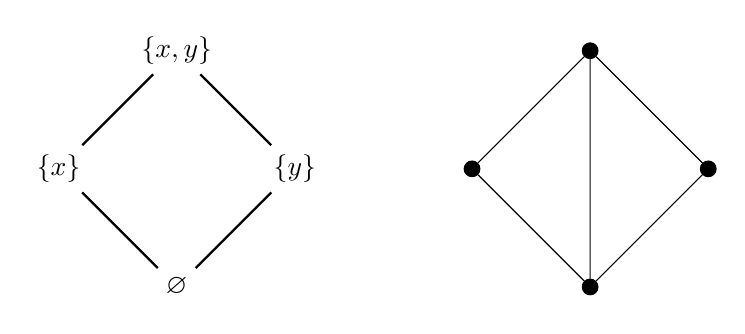
\begin{tikzpicture}[scale=1.5]

  % poset
  \draw (-1cm,0cm) node (v2) {$\{x\}$};
  \draw (1cm,0cm)  node (v3) { $\{y\}$ };
  \draw (0cm,-1cm) node (v4) {$\varnothing$};
  \draw (0cm,1cm)  node (v1) {$\{x,y\}$};

  \draw[thick]  (v1) edge (v2);
  \draw[thick]  (v3) edge (v1);
  \draw[thick]  (v3) edge (v4);
  \draw[thick]  (v2) edge (v4);

  % graph
  \node[draw,circle,inner sep=2pt,fill,label distance=1cm] (v1g) at (3.5,1) {};
  \node[draw,circle,inner sep=2pt,fill,label distance=1cm] (v2g) at (3.5,-1) {};
  \node[draw,circle,inner sep=2pt,fill,label distance=1cm] (v3g) at (4.5,0) {};
  \node[draw,circle,inner sep=2pt,fill,label distance=1cm] (v4g) at (2.5,0) {};
  \draw  (v1g) edge (v2g);
  \draw  (v1g) edge (v4g);
  \draw  (v4g) edge (v2g);
  \draw  (v1g) edge (v3g);
  \draw  (v3g) edge (v2g);

\end{tikzpicture}
\end{scaletikzpicturetowidth}

\caption{On the left, Hasse diagram of a poset of the power set of 2 elements ordered by inclusion.
On the right, the comparability graph of this poset.}
\label{fig:hasse}
\end{figure}

\subsubsection{Disks}

A disk graph $G$ is a graph that is an intersection graph of disks on the plane, when the size
of the disk is unitary, we talk about unit disk graphs. This class of graphs
is important for this thesis, as thin strip graphs are a sub-class of
unit disk graphs.

We will refer to the unit disk graph class as UDG and an example of a realization
can be found in the figure \ref{fig:udg}.

\paragraph{Induced forbidden subgraphs} The characterization of this class with respect to
its induced forbidden subgraphs has been studied \cite{atminasForbiddenInducedSubgraphs2016}.

\begin{theorem}[Atminas-Zamaraev]
  For every integer $k > 1$, $\overline{K_2 + C_{2k+1}}$ is a minimal induced subgraph of UDG.
\end{theorem}

\begin{theorem}[Atminas-Zamaraev]
  For every integer $k > 4$, $\overline{C_{2k}}$ is a minimal induced subgraph of UDG.
\end{theorem}

\begin{figure}
\centering

\begin{scaletikzpicturetowidth}{\textwidth}
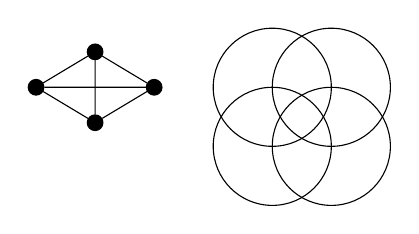
\begin{tikzpicture}[scale=1.5]

  \draw (-0.5,2.5) circle [radius=0.5];
  \draw (0,2.5) circle [radius=0.5];
  \draw (-0.5,2) circle [radius=0.5];
  \draw (0,2) circle [radius=0.5];


  \node[draw,circle,inner sep=2pt,fill,label distance=1cm] (v1) at (-2.5,2.5) {};

  \node[draw,circle,inner sep=2pt,fill,label distance=1cm] (v2) at (-2,2.2) {};
  \node[draw,circle,inner sep=2pt,fill,label distance=1cm] (v3) at (-2,2.8) {};
  \node[draw,circle,inner sep=2pt,fill,label distance=1cm] (v4) at (-1.5,2.5) {};

  \draw  (v3) edge (v2);
  \draw  (v4) edge (v1);
  \draw  (v3) edge (v1);
  \draw  (v4) edge (v2);
  \draw  (v3) edge (v4);
  \draw  (v1) edge (v2);

\end{tikzpicture}
\end{scaletikzpicturetowidth}

\caption{Realization of a UDG (Unit Disk Graph).}
\label{fig:udg}
\end{figure}

%\input{chap1/complexity}
%%% This is an example first chapter.  You should put chapter/appendix that you
%% write into a separate file, and add a line \include{yourfilename} to
%% main.tex, where `yourfilename.tex' is the name of the chapter/appendix file.
%% You can process specific files by typing their names in at the
%% \files=
%% prompt when you run the file main.tex through LaTeX.
\section{Geometry}
\label{sec:geom}

\begin{defn}
  $\text{dist}(a,b)$ denotes the distance between the points $a$ and $b$ and is calculated with:

  $$\text{dist}(a,b) = \sqrt{(a_x - b_x)^2 + (a_y - b_y)^2}$$
\end{defn}

The intersection of convex objects is a matter well studied for multiple
subjects. In our case, it is interesting to know some properties about
the intersection of disks, those ones being convex objects.

A set $S$ is convex if:
$$\forall p,q \in S\  \forall \lambda \in [0,1]: (1-\lambda)p + \lambda q \in S$$

\subsection{Stabbing}
A \textit{stabbing} is a point that traverses a set of intersecting objects. A lot of
research has been done \cite{schlipf2013stabbing} on the minimal amount of stabbings to
cover every object in a set. Stabbings can also be done with more complex structures
than points, in that case we are talking about \textit{coverings}.

\begin{theorem}[Helly]
  Given a set $Q$ of objects in $\mathbb{R}^d$, if for each subset of $Q$ of
  size $d+1$ their intersection is non empty, then $\bigcap_{q \in Q} \neq
  \varnothing$. \cite{Helly1923175}
\end{theorem}

\begin{theorem}
  The problem that for a set of $n$ disks whether there exists a regular n-gon
  whose vertices stab every disk of the set can be decided in $O(n^{10.5} / \sqrt{\log(n)})$ \cite{schlipf2013stabbing}
\end{theorem}

\subsection{Coin graphs}

Penny graphs can be defined as disk graphs where the disks can just touch each
other without overlapping. A famous theorem is derived from this class of graphs:
the circle packing theorem.

\begin{theorem}[Circle packing theorem]
  The circle packing theorem states that every simple connected planar graph
  $G$ is a penny graph. \cite{doi:10.1137/0406017}
\end{theorem}

\begin{corollary}
  Planar graphs $\subseteq$ disk graphs \cite{spinradEfficientGraphRepresentations2012}.
\end{corollary}

\begin{figure}
\centering
\includegraphics[width=1.0\textwidth]{res/circle_packing}
\caption{Circle packing of a planar graph. \cite{nachmiasPlanarMapsRandom2016}}
\label{fig:circle}
\end{figure}


\section{Graph theory}

A \emph{graph} is defined as a tuple $G = (V,E)$ where $V$ is the set of \emph{vertices} and $E$. When the the set of \emph{edges}, where $E = \binom{V}{2}$. If two vertices are share the same edge $e$ they are called \emph{adjacent} and also the \emph{endpoints} of $e$. A \emph{subgraph} $H = (V', E')$ of a graph $G$ is a graph such that $V' \subseteq V$ and $E' \subseteq E$. An \emph{induced subgraph} of a graph is a subgraph $H$ of a graph $G$ such that for every edge of $G$ is also in $H$ if its two endpoints are in $V'$. A \emph{clique} is a subgraph such that every vertex is adjacent to each other. A graph that is also a clique is called a \emph{complete graph} and it is denoted as $K_n$. A graph is \emph{bipartite} if there exist two disjoint subsets of the vertex set $A \cup B = V$ such that two vertices of the same subset are not adjacent. A \emph{complete bipartite graph} $K_{n,m}$ is a bipartite graph such that $v \in A$ and $w \in B$ implies $vw \in E$ where $n$ and $m$ are the size of each bipartition.

A \emph{path} $P_n = v_1\dots v_{n+1}$ of a graph is a sequence of $n$ vertices such that two consequent vertices are adjacent. A \emph{cycle} is a path $C_n = v_1\dots v_nv_{n+1}$ such that $v_1=v_{n+1}$. A graph is \emph{connected} if there exists a path between every pair of vertices. A \emph{chord} of a cycle $C_n$ with $n \geqslant 4$ is an edge that connects two non adjacent vertices of the cycle. A graph is \emph{chordal} if there is a chord in every cycle bigger than four.

\subsection{Intersection graphs}

\begin{figure}
\centering

\begin{scaletikzpicturetowidth}{\textwidth}
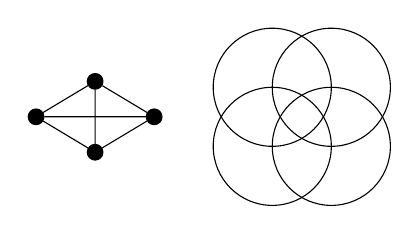
\begin{tikzpicture}[scale=1.5]

  \draw (-0.5,2.5) circle [radius=0.5];
  \draw (0,2.5) circle [radius=0.5];
  \draw (-0.5,2) circle [radius=0.5];
  \draw (0,2) circle [radius=0.5];


  \node[draw,circle,inner sep=2pt,fill,label distance=1cm] (v1) at (-2.5,2.25) {};

  \node[draw,circle,inner sep=2pt,fill,label distance=1cm] (v2) at (-2,1.95) {};
  \node[draw,circle,inner sep=2pt,fill,label distance=1cm] (v3) at (-2,2.55) {};
  \node[draw,circle,inner sep=2pt,fill,label distance=1cm] (v4) at (-1.5,2.25) {};

  \draw  (v3) edge (v2);
  \draw  (v4) edge (v1);
  \draw  (v3) edge (v1);
  \draw  (v4) edge (v2);
  \draw  (v3) edge (v4);
  \draw  (v1) edge (v2);

\end{tikzpicture}
\end{scaletikzpicturetowidth}

\caption{Realization of a UDG (unit disk graph).}
\label{fig:udg}
\end{figure}


An \emph{intersection graph} is a graph $G = (\zeta,E)$ of a collection of objects $\zeta$ is a graph such that $v,w \in \zeta$ and $v \cup w \neq \varnothing$ implies that $vw \in E$. An \emph{interval graph} is an intersection graph of intervals on the plane; when the size of the intervals is equal they are called \emph{unit interval graphs}. A \emph{unit disk graph} is an intersection graph of disks on a plane that have the same diameter - you can find an example in Figure \ref{fig:udg}.

\section{Order and set theory}

The \emph{powerset} $\powerset(S)$ of a set $S$ is the set of subsets of $S$. A \emph{partial order} is a binary relation $\leqslant$ over a set $A$ satisfying three axioms:

\begin{itemize}
  \item if $a \leqslant b$ and $b \leqslant a$ then $a = b$ (\emph{antisymmetry}).
  \item if $a \leqslant b$ and $b \leqslant c$ then $a \leqslant c$ (\emph{transitivity}).
  \item $a \leqslant a$ (\emph{reflexivity}).
\end{itemize}

\begin{figure}
\centering

\begin{scaletikzpicturetowidth}{\textwidth}
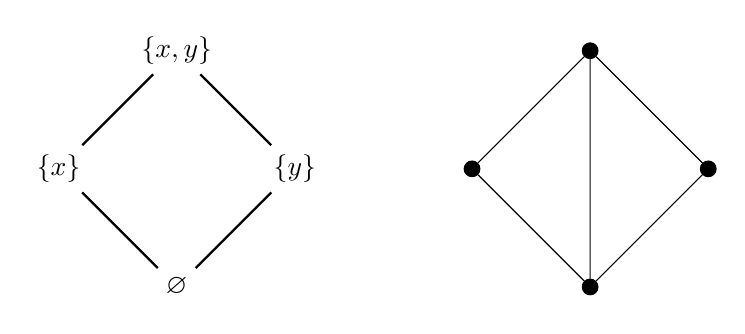
\begin{tikzpicture}[scale=1.5]

  % poset
  \draw (-1cm,0cm) node (v2) {$\{x\}$};
  \draw (1cm,0cm)  node (v3) { $\{y\}$ };
  \draw (0cm,-1cm) node (v4) {$\varnothing$};
  \draw (0cm,1cm)  node (v1) {$\{x,y\}$};

  \draw[thick]  (v1) edge (v2);
  \draw[thick]  (v3) edge (v1);
  \draw[thick]  (v3) edge (v4);
  \draw[thick]  (v2) edge (v4);

  % graph
  \node[draw,circle,inner sep=2pt,fill,label distance=1cm] (v1g) at (3.5,1) {};
  \node[draw,circle,inner sep=2pt,fill,label distance=1cm] (v2g) at (3.5,-1) {};
  \node[draw,circle,inner sep=2pt,fill,label distance=1cm] (v3g) at (4.5,0) {};
  \node[draw,circle,inner sep=2pt,fill,label distance=1cm] (v4g) at (2.5,0) {};
  \draw  (v1g) edge (v2g);
  \draw  (v1g) edge (v4g);
  \draw  (v4g) edge (v2g);
  \draw  (v1g) edge (v3g);
  \draw  (v3g) edge (v2g);

\end{tikzpicture}
\end{scaletikzpicturetowidth}

\caption{On the left, Hasse diagram of a poset of the power set of 2 elements ordered by inclusion.
On the right, the comparability graph of this poset.}
\label{fig:hasse}
\end{figure}

In the other side, a \emph{total order} is a partial order where the reflexivity order is replaced by the \emph{connexity} property -- $a \leq b\ \text{or}\  b \leq a$. A \emph{partially ordered set} (or \emph{poset}) $(S,\leqslant)$ is a set such that the elements of $S$ are partially ordered by the relation $\leqslant$. A good way to represent a poset is the \emph{Hasse diagram} (figure \ref{fig:hasse}).

\subsection{Comparability graphs}

A \emph{spanning order} $(V,<)$ on a graph $G = (V,E)$ is a total order on $V$ such that for any three vertices $u < v < w$:

  $$uw \in E \to uv \in E\ \text{or}\ vw \in E$$

The class of comparability graphs are built on the ideas of order theory. A graph $G$ is a \emph{comparability graph} if there exists a partial order $\leqslant$ such that $uv \in E \Leftrightarrow v \leqslant w\  \text{or}\  w \leqslant v$.

\section{Geometry}

\chapter{Background}
\label{chap:background}

In this chapter we review some definitions and notations of the background knowledge of this thesis. We limit ourselves to the basic notations used during the work. Nevertheless, the bibliography of each subject will be referenced for further details about the topic.

%\todo{Text about background intro}

%%% This is an example first chapter.  You should put chapter/appendix that you
%% write into a separate file, and add a line \include{yourfilename} to
%% main.tex, where `yourfilename.tex' is the name of the chapter/appendix file.
%% You can process specific files by typing their names in at the
%% \files=
%% prompt when you run the file main.tex through LaTeX.
\section{Graphs and intersections}
\label{sec:graphs}


\subsection{Graphs}

A graph $G$ is defined as $G = (V,E)$, where $V$ is the set of vertices and $E$ the set of
edges, where $E \subseteq \binom{V}{2}$. The vertices $v,w \in V$ such that $e = vw \in E$
links are called the \textit{endpoints} of $e$.

\begin{defn}
  An embedding of a graph $G$ into a surface $\Sigma$ is a mapping of $G$ in
  $\Sigma$ where the vertices correspond to distinct points and the edges
  correspond to simple arcs connecting the images of their endpoints.
  \cite{goyalGraphEmbeddingTechniques2017}.
\end{defn}

A graph $G$ is planar if there is an embedding of this graph that does not have
any crossing between the edges.

\begin{defn}
  Let $G = (V,E)$ and $S \subset V$, an induced subgraph is a graph $H$ of $G$ whose
  vertex set is $S$ and its edge set $F = \{vw : v,w \in S, vw \in E\}$.
\end{defn}

\begin{defn}
  Let $G = (V,E)$ its complement graph $\overline{G}$ is the graph such that its edge set
  is defined as: $\{vw: v,w\in V, vw\notin E\}$.
\end{defn}

\begin{defn}
  $H$ is called a \textit{minor} of $G$ if $H$ can be constructed by deleting edges and vertices,
  or contracting edges.
\end{defn}

\begin{theorem}[Kuratowski]
  \label{theo:kura}
  A graph $G$ is planar if and only if it does not contain $K_5$ or $K_{3,3}$ as a minor or
  a induced subgraph.
\end{theorem}

\begin{defn}
  A path $P_n$ in a graph $G$ is a sequence of vertices $v_1v_2v_3\dots v_n$ such
  that $v_iv_{i+1} \in E$.
\end{defn}

\begin{defn}
  A cycle $C_n$ in a graph $G = (V,E)$ is a path $v_1\dots v_n$ such that $v_1 = v_n$.
\end{defn}

\begin{defn}
  A chord of a cycle $C_n$ with $n \geq 4 $ is an edge that connects two non consecutive vertices
  of $C_n$.
\end{defn}

\begin{defn}
  A triangular chord of a cycle is a chord that will create a new triangle ($C_3$).
\end{defn}


\begin{defn}
  A graph $G = (V,E)$ is complete if every pair of distinct $v_1,v_2 \in V$ are
  adjacent. This is denoted $K_n$ with $n$ the size of the graph. If $G$ is an
  induced graph of $H$ then $G$ is a clique of $H$.
\end{defn}

\begin{defn}
  A graph $G$ is bipartite if there exist two disjoint subsets $A,B \subset V$ such
  that $A\cup B = V$ and each edge $e\in E$ has an endpoint on $A$ and the
  another on $B$.
\end{defn}

\begin{defn}
  A bipartite graph $G$ with bipartitions $A$ and $B$ is complete bipartite if
  every pair of vertices $v\in A, w\in B$ are adjacent. It is denoted as $K_{n,m}$,
  being $n$ and $m$ the size of each bipartition.
\end{defn}

Some graphs can be characterized with properties. A property of a graph is a property that
is preserved under all its isomophisms. These properties are called \textit{hereditary} if they
are also preserved under all its induced subgraphs; they are called \textit{minor-hereditary} if they are
also preserved under its minors (e.g. Kuratowski's planar graph characterization [\ref{theo:kura}]).

\begin{defn}
  An forbidden induced subgraph (minor) of a graph class $X$ is a graph such that if it is the induced
  subgraph (minor) of a graph $G$, we know that $G \notin X$.
\end{defn}

The coloration of a graph is a color assignment to each vertex such that the color
of the two endpoints of every edge of the graph is different.

\begin{defn}
  The chromatic number of a graph $\chi(G)$ is the smallest number of colors needed to
  have an acceptable coloration of $G$.
\end{defn}

\begin{defn}
  The clique number of a graph $\omega(G)$ is the size of the biggest clique of $G$. We
  can observe that for every graph: $\chi(G) \geq \omega(G)$.
\end{defn}

\begin{defn}
  A perfect graph is a graph that respects this condition for every induced subgraph:
  $$ \omega(G) = \chi(G)$$
\end{defn}

\begin{theorem}[Lovasz]
  $G$ is perfect if and only if $\overline{G}$ is perfect.
\end{theorem}

\subsection{Intersection graphs}

\begin{defn}
The \textit{intersection graph} of a collection $\zeta$ of objects is the graph
$(\zeta,E)$ such that $c_1c_2\in E \Leftrightarrow c_1 \cap c_2 \neq \varnothing$.
\end{defn}

An intersection can be seen as a relationship between two objects. In this thesis, it will be important to define these relations more formally to characterize intersection graphs.

\begin{defn}
  A partial order is a binary relation $\leq$ over a set $A$ satisfying these axioms:
  \begin{itemize}
    \item if $a \leq b$ and $b \leq a$ then $a = b$ (antisymmetry).
    \item if $a \leq b$ and $b \leq c$ then $a \leq c$ (transitivity).
    \item $a \leq a$ (reflexivity).
  \end{itemize}
\end{defn}

\begin{defn}
  A total order is a partial order where the reflexivity order is replaced by the connex property:
  $$a \leq b\ \text{or}\  b \leq a$$
\end{defn}

\begin{defn}
   A partially ordered set or poset  $(S,\leq)$ where $S$ a set and $\leq$ a partial
   order on $S$.
\end{defn}

\begin{defn}
  A spanning order $(V,<)$ of a graph $G = (V,E)$ is a total order on $V$ such that for any three vertices $u < v < w$:

  $$uw \in E \to uv \in E\ \text{or}\ vw \in E$$
\end{defn}


\begin{defn}
  A graph $G = (V,E)$ is a comparibility graph if there exists a partial order
  $\leq$ such that $vw \in E \Leftrightarrow v \leq w$ or $w \leq v$.
  Equivalently, $G$ is a comparability graph if it is the comparability graph of
  a poset. For example, the Hasse diagram (figure \ref{fig:hasse}) is a
  comparability graph where the relation is inclusion.
\end{defn}

\begin{defn}
  A graph $G = (V,E)$ is a co-comparability graph if its complement is a comparability graph.
\end{defn}

There are multiple characterizations for the co-comparability graph class; we will see one that uses a poset to characterize it:

\begin{theorem}[Damaschke \cite{damaschkeDistancesCocomparabilityGraphs1992}]
  \label{theo:spanning}
  A graph $G$ is a co-comparability graph if and only if it has a spanning order.
\end{theorem}


\begin{figure}
\centering

\begin{scaletikzpicturetowidth}{\textwidth}
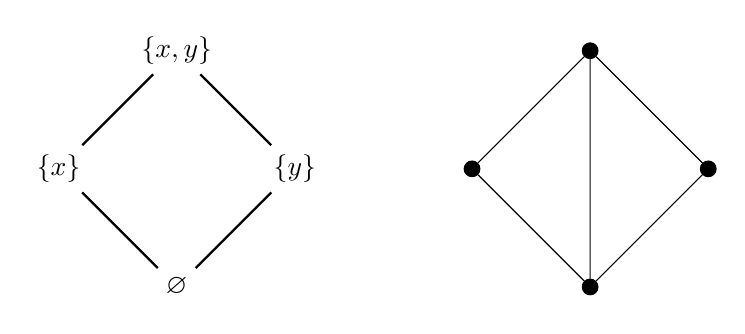
\begin{tikzpicture}[scale=1.5]

  % poset
  \draw (-1cm,0cm) node (v2) {$\{x\}$};
  \draw (1cm,0cm)  node (v3) { $\{y\}$ };
  \draw (0cm,-1cm) node (v4) {$\varnothing$};
  \draw (0cm,1cm)  node (v1) {$\{x,y\}$};

  \draw[thick]  (v1) edge (v2);
  \draw[thick]  (v3) edge (v1);
  \draw[thick]  (v3) edge (v4);
  \draw[thick]  (v2) edge (v4);

  % graph
  \node[draw,circle,inner sep=2pt,fill,label distance=1cm] (v1g) at (3.5,1) {};
  \node[draw,circle,inner sep=2pt,fill,label distance=1cm] (v2g) at (3.5,-1) {};
  \node[draw,circle,inner sep=2pt,fill,label distance=1cm] (v3g) at (4.5,0) {};
  \node[draw,circle,inner sep=2pt,fill,label distance=1cm] (v4g) at (2.5,0) {};
  \draw  (v1g) edge (v2g);
  \draw  (v1g) edge (v4g);
  \draw  (v4g) edge (v2g);
  \draw  (v1g) edge (v3g);
  \draw  (v3g) edge (v2g);

\end{tikzpicture}
\end{scaletikzpicturetowidth}

\caption{On the left, Hasse diagram of a poset of the power set of 2 elements ordered by inclusion.
On the right, the comparability graph of this poset.}
\label{fig:hasse}
\end{figure}

\subsubsection{Disks}

A disk graph $G$ is a graph that is an intersection graph of disks on the plane, when the size
of the disk is unitary, we talk about unit disk graphs. This class of graphs
is important for this thesis, as thin strip graphs are a sub-class of
unit disk graphs.

We will refer to the unit disk graph class as UDG and an example of a realization
can be found in the figure \ref{fig:udg}.

\paragraph{Induced forbidden subgraphs} The characterization of this class with respect to
its induced forbidden subgraphs has been studied \cite{atminasForbiddenInducedSubgraphs2016}.

\begin{theorem}[Atminas-Zamaraev]
  For every integer $k > 1$, $\overline{K_2 + C_{2k+1}}$ is a minimal induced subgraph of UDG.
\end{theorem}

\begin{theorem}[Atminas-Zamaraev]
  For every integer $k > 4$, $\overline{C_{2k}}$ is a minimal induced subgraph of UDG.
\end{theorem}

\begin{figure}
\centering

\begin{scaletikzpicturetowidth}{\textwidth}
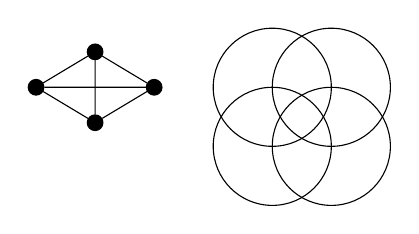
\begin{tikzpicture}[scale=1.5]

  \draw (-0.5,2.5) circle [radius=0.5];
  \draw (0,2.5) circle [radius=0.5];
  \draw (-0.5,2) circle [radius=0.5];
  \draw (0,2) circle [radius=0.5];


  \node[draw,circle,inner sep=2pt,fill,label distance=1cm] (v1) at (-2.5,2.5) {};

  \node[draw,circle,inner sep=2pt,fill,label distance=1cm] (v2) at (-2,2.2) {};
  \node[draw,circle,inner sep=2pt,fill,label distance=1cm] (v3) at (-2,2.8) {};
  \node[draw,circle,inner sep=2pt,fill,label distance=1cm] (v4) at (-1.5,2.5) {};

  \draw  (v3) edge (v2);
  \draw  (v4) edge (v1);
  \draw  (v3) edge (v1);
  \draw  (v4) edge (v2);
  \draw  (v3) edge (v4);
  \draw  (v1) edge (v2);

\end{tikzpicture}
\end{scaletikzpicturetowidth}

\caption{Realization of a UDG (Unit Disk Graph).}
\label{fig:udg}
\end{figure}

%\input{chap1/complexity}
%%% This is an example first chapter.  You should put chapter/appendix that you
%% write into a separate file, and add a line \include{yourfilename} to
%% main.tex, where `yourfilename.tex' is the name of the chapter/appendix file.
%% You can process specific files by typing their names in at the
%% \files=
%% prompt when you run the file main.tex through LaTeX.
\section{Geometry}
\label{sec:geom}

\begin{defn}
  $\text{dist}(a,b)$ denotes the distance between the points $a$ and $b$ and is calculated with:

  $$\text{dist}(a,b) = \sqrt{(a_x - b_x)^2 + (a_y - b_y)^2}$$
\end{defn}

The intersection of convex objects is a matter well studied for multiple
subjects. In our case, it is interesting to know some properties about
the intersection of disks, those ones being convex objects.

A set $S$ is convex if:
$$\forall p,q \in S\  \forall \lambda \in [0,1]: (1-\lambda)p + \lambda q \in S$$

\subsection{Stabbing}
A \textit{stabbing} is a point that traverses a set of intersecting objects. A lot of
research has been done \cite{schlipf2013stabbing} on the minimal amount of stabbings to
cover every object in a set. Stabbings can also be done with more complex structures
than points, in that case we are talking about \textit{coverings}.

\begin{theorem}[Helly]
  Given a set $Q$ of objects in $\mathbb{R}^d$, if for each subset of $Q$ of
  size $d+1$ their intersection is non empty, then $\bigcap_{q \in Q} \neq
  \varnothing$. \cite{Helly1923175}
\end{theorem}

\begin{theorem}
  The problem that for a set of $n$ disks whether there exists a regular n-gon
  whose vertices stab every disk of the set can be decided in $O(n^{10.5} / \sqrt{\log(n)})$ \cite{schlipf2013stabbing}
\end{theorem}

\subsection{Coin graphs}

Penny graphs can be defined as disk graphs where the disks can just touch each
other without overlapping. A famous theorem is derived from this class of graphs:
the circle packing theorem.

\begin{theorem}[Circle packing theorem]
  The circle packing theorem states that every simple connected planar graph
  $G$ is a penny graph. \cite{doi:10.1137/0406017}
\end{theorem}

\begin{corollary}
  Planar graphs $\subseteq$ disk graphs \cite{spinradEfficientGraphRepresentations2012}.
\end{corollary}

\begin{figure}
\centering
\includegraphics[width=1.0\textwidth]{res/circle_packing}
\caption{Circle packing of a planar graph. \cite{nachmiasPlanarMapsRandom2016}}
\label{fig:circle}
\end{figure}


\section{Graph theory}

A \emph{graph} is defined as a tuple $G = (V,E)$ where $V$ is the set of \emph{vertices} and $E$. When the the set of \emph{edges}, where $E = \binom{V}{2}$. If two vertices are share the same edge $e$ they are called \emph{adjacent} and also the \emph{endpoints} of $e$. A \emph{subgraph} $H = (V', E')$ of a graph $G$ is a graph such that $V' \subseteq V$ and $E' \subseteq E$. An \emph{induced subgraph} of a graph is a subgraph $H$ of a graph $G$ such that for every edge of $G$ is also in $H$ if its two endpoints are in $V'$. A \emph{clique} is a subgraph such that every vertex is adjacent to each other. A graph that is also a clique is called a \emph{complete graph} and it is denoted as $K_n$. A graph is \emph{bipartite} if there exist two disjoint subsets of the vertex set $A \cup B = V$ such that two vertices of the same subset are not adjacent. A \emph{complete bipartite graph} $K_{n,m}$ is a bipartite graph such that $v \in A$ and $w \in B$ implies $vw \in E$ where $n$ and $m$ are the size of each bipartition.

A \emph{path} $P_n = v_1\dots v_{n+1}$ of a graph is a sequence of $n$ vertices such that two consequent vertices are adjacent. A \emph{cycle} is a path $C_n = v_1\dots v_nv_{n+1}$ such that $v_1=v_{n+1}$. A graph is \emph{connected} if there exists a path between every pair of vertices. A \emph{chord} of a cycle $C_n$ with $n \geqslant 4$ is an edge that connects two non adjacent vertices of the cycle. A graph is \emph{chordal} if there is a chord in every cycle bigger than four.

\subsection{Intersection graphs}

\begin{figure}
\centering

\begin{scaletikzpicturetowidth}{\textwidth}
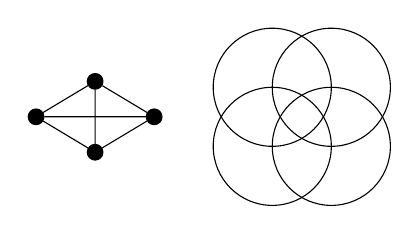
\begin{tikzpicture}[scale=1.5]

  \draw (-0.5,2.5) circle [radius=0.5];
  \draw (0,2.5) circle [radius=0.5];
  \draw (-0.5,2) circle [radius=0.5];
  \draw (0,2) circle [radius=0.5];


  \node[draw,circle,inner sep=2pt,fill,label distance=1cm] (v1) at (-2.5,2.25) {};

  \node[draw,circle,inner sep=2pt,fill,label distance=1cm] (v2) at (-2,1.95) {};
  \node[draw,circle,inner sep=2pt,fill,label distance=1cm] (v3) at (-2,2.55) {};
  \node[draw,circle,inner sep=2pt,fill,label distance=1cm] (v4) at (-1.5,2.25) {};

  \draw  (v3) edge (v2);
  \draw  (v4) edge (v1);
  \draw  (v3) edge (v1);
  \draw  (v4) edge (v2);
  \draw  (v3) edge (v4);
  \draw  (v1) edge (v2);

\end{tikzpicture}
\end{scaletikzpicturetowidth}

\caption{Realization of a UDG (unit disk graph).}
\label{fig:udg}
\end{figure}


An \emph{intersection graph} is a graph $G = (\zeta,E)$ of a collection of objects $\zeta$ is a graph such that $v,w \in \zeta$ and $v \cup w \neq \varnothing$ implies that $vw \in E$. An \emph{interval graph} is an intersection graph of intervals on the plane; when the size of the intervals is equal they are called \emph{unit interval graphs}. A \emph{unit disk graph} is an intersection graph of disks on a plane that have the same diameter - you can find an example in Figure \ref{fig:udg}.

\section{Order and set theory}

The \emph{powerset} $\powerset(S)$ of a set $S$ is the set of subsets of $S$. A \emph{partial order} is a binary relation $\leqslant$ over a set $A$ satisfying three axioms:

\begin{itemize}
  \item if $a \leqslant b$ and $b \leqslant a$ then $a = b$ (\emph{antisymmetry}).
  \item if $a \leqslant b$ and $b \leqslant c$ then $a \leqslant c$ (\emph{transitivity}).
  \item $a \leqslant a$ (\emph{reflexivity}).
\end{itemize}

\begin{figure}
\centering

\begin{scaletikzpicturetowidth}{\textwidth}
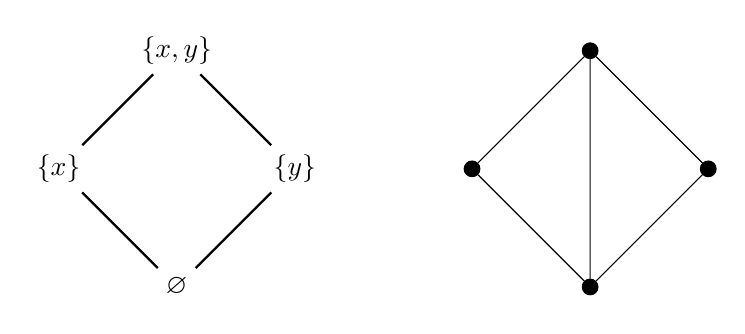
\begin{tikzpicture}[scale=1.5]

  % poset
  \draw (-1cm,0cm) node (v2) {$\{x\}$};
  \draw (1cm,0cm)  node (v3) { $\{y\}$ };
  \draw (0cm,-1cm) node (v4) {$\varnothing$};
  \draw (0cm,1cm)  node (v1) {$\{x,y\}$};

  \draw[thick]  (v1) edge (v2);
  \draw[thick]  (v3) edge (v1);
  \draw[thick]  (v3) edge (v4);
  \draw[thick]  (v2) edge (v4);

  % graph
  \node[draw,circle,inner sep=2pt,fill,label distance=1cm] (v1g) at (3.5,1) {};
  \node[draw,circle,inner sep=2pt,fill,label distance=1cm] (v2g) at (3.5,-1) {};
  \node[draw,circle,inner sep=2pt,fill,label distance=1cm] (v3g) at (4.5,0) {};
  \node[draw,circle,inner sep=2pt,fill,label distance=1cm] (v4g) at (2.5,0) {};
  \draw  (v1g) edge (v2g);
  \draw  (v1g) edge (v4g);
  \draw  (v4g) edge (v2g);
  \draw  (v1g) edge (v3g);
  \draw  (v3g) edge (v2g);

\end{tikzpicture}
\end{scaletikzpicturetowidth}

\caption{On the left, Hasse diagram of a poset of the power set of 2 elements ordered by inclusion.
On the right, the comparability graph of this poset.}
\label{fig:hasse}
\end{figure}

In the other side, a \emph{total order} is a partial order where the reflexivity order is replaced by the \emph{connexity} property -- $a \leq b\ \text{or}\  b \leq a$. A \emph{partially ordered set} (or \emph{poset}) $(S,\leqslant)$ is a set such that the elements of $S$ are partially ordered by the relation $\leqslant$. A good way to represent a poset is the \emph{Hasse diagram} (figure \ref{fig:hasse}).

\subsection{Comparability graphs}

A \emph{spanning order} $(V,<)$ on a graph $G = (V,E)$ is a total order on $V$ such that for any three vertices $u < v < w$:

  $$uw \in E \to uv \in E\ \text{or}\ vw \in E$$

The class of comparability graphs are built on the ideas of order theory. A graph $G$ is a \emph{comparability graph} if there exists a partial order $\leqslant$ such that $uv \in E \Leftrightarrow v \leqslant w\  \text{or}\  w \leqslant v$.

\section{Geometry}

\chapter{Background}
\label{chap:background}

In this chapter we review some definitions and notations of the background knowledge of this thesis. We limit ourselves to the basic notations used during the work. Nevertheless, the bibliography of each subject will be referenced for further details about the topic.

%\todo{Text about background intro}

%%% This is an example first chapter.  You should put chapter/appendix that you
%% write into a separate file, and add a line \include{yourfilename} to
%% main.tex, where `yourfilename.tex' is the name of the chapter/appendix file.
%% You can process specific files by typing their names in at the
%% \files=
%% prompt when you run the file main.tex through LaTeX.
\section{Graphs and intersections}
\label{sec:graphs}


\subsection{Graphs}

A graph $G$ is defined as $G = (V,E)$, where $V$ is the set of vertices and $E$ the set of
edges, where $E \subseteq \binom{V}{2}$. The vertices $v,w \in V$ such that $e = vw \in E$
links are called the \textit{endpoints} of $e$.

\begin{defn}
  An embedding of a graph $G$ into a surface $\Sigma$ is a mapping of $G$ in
  $\Sigma$ where the vertices correspond to distinct points and the edges
  correspond to simple arcs connecting the images of their endpoints.
  \cite{goyalGraphEmbeddingTechniques2017}.
\end{defn}

A graph $G$ is planar if there is an embedding of this graph that does not have
any crossing between the edges.

\begin{defn}
  Let $G = (V,E)$ and $S \subset V$, an induced subgraph is a graph $H$ of $G$ whose
  vertex set is $S$ and its edge set $F = \{vw : v,w \in S, vw \in E\}$.
\end{defn}

\begin{defn}
  Let $G = (V,E)$ its complement graph $\overline{G}$ is the graph such that its edge set
  is defined as: $\{vw: v,w\in V, vw\notin E\}$.
\end{defn}

\begin{defn}
  $H$ is called a \textit{minor} of $G$ if $H$ can be constructed by deleting edges and vertices,
  or contracting edges.
\end{defn}

\begin{theorem}[Kuratowski]
  \label{theo:kura}
  A graph $G$ is planar if and only if it does not contain $K_5$ or $K_{3,3}$ as a minor or
  a induced subgraph.
\end{theorem}

\begin{defn}
  A path $P_n$ in a graph $G$ is a sequence of vertices $v_1v_2v_3\dots v_n$ such
  that $v_iv_{i+1} \in E$.
\end{defn}

\begin{defn}
  A cycle $C_n$ in a graph $G = (V,E)$ is a path $v_1\dots v_n$ such that $v_1 = v_n$.
\end{defn}

\begin{defn}
  A chord of a cycle $C_n$ with $n \geq 4 $ is an edge that connects two non consecutive vertices
  of $C_n$.
\end{defn}

\begin{defn}
  A triangular chord of a cycle is a chord that will create a new triangle ($C_3$).
\end{defn}


\begin{defn}
  A graph $G = (V,E)$ is complete if every pair of distinct $v_1,v_2 \in V$ are
  adjacent. This is denoted $K_n$ with $n$ the size of the graph. If $G$ is an
  induced graph of $H$ then $G$ is a clique of $H$.
\end{defn}

\begin{defn}
  A graph $G$ is bipartite if there exist two disjoint subsets $A,B \subset V$ such
  that $A\cup B = V$ and each edge $e\in E$ has an endpoint on $A$ and the
  another on $B$.
\end{defn}

\begin{defn}
  A bipartite graph $G$ with bipartitions $A$ and $B$ is complete bipartite if
  every pair of vertices $v\in A, w\in B$ are adjacent. It is denoted as $K_{n,m}$,
  being $n$ and $m$ the size of each bipartition.
\end{defn}

Some graphs can be characterized with properties. A property of a graph is a property that
is preserved under all its isomophisms. These properties are called \textit{hereditary} if they
are also preserved under all its induced subgraphs; they are called \textit{minor-hereditary} if they are
also preserved under its minors (e.g. Kuratowski's planar graph characterization [\ref{theo:kura}]).

\begin{defn}
  An forbidden induced subgraph (minor) of a graph class $X$ is a graph such that if it is the induced
  subgraph (minor) of a graph $G$, we know that $G \notin X$.
\end{defn}

The coloration of a graph is a color assignment to each vertex such that the color
of the two endpoints of every edge of the graph is different.

\begin{defn}
  The chromatic number of a graph $\chi(G)$ is the smallest number of colors needed to
  have an acceptable coloration of $G$.
\end{defn}

\begin{defn}
  The clique number of a graph $\omega(G)$ is the size of the biggest clique of $G$. We
  can observe that for every graph: $\chi(G) \geq \omega(G)$.
\end{defn}

\begin{defn}
  A perfect graph is a graph that respects this condition for every induced subgraph:
  $$ \omega(G) = \chi(G)$$
\end{defn}

\begin{theorem}[Lovasz]
  $G$ is perfect if and only if $\overline{G}$ is perfect.
\end{theorem}

\subsection{Intersection graphs}

\begin{defn}
The \textit{intersection graph} of a collection $\zeta$ of objects is the graph
$(\zeta,E)$ such that $c_1c_2\in E \Leftrightarrow c_1 \cap c_2 \neq \varnothing$.
\end{defn}

An intersection can be seen as a relationship between two objects. In this thesis, it will be important to define these relations more formally to characterize intersection graphs.

\begin{defn}
  A partial order is a binary relation $\leq$ over a set $A$ satisfying these axioms:
  \begin{itemize}
    \item if $a \leq b$ and $b \leq a$ then $a = b$ (antisymmetry).
    \item if $a \leq b$ and $b \leq c$ then $a \leq c$ (transitivity).
    \item $a \leq a$ (reflexivity).
  \end{itemize}
\end{defn}

\begin{defn}
  A total order is a partial order where the reflexivity order is replaced by the connex property:
  $$a \leq b\ \text{or}\  b \leq a$$
\end{defn}

\begin{defn}
   A partially ordered set or poset  $(S,\leq)$ where $S$ a set and $\leq$ a partial
   order on $S$.
\end{defn}

\begin{defn}
  A spanning order $(V,<)$ of a graph $G = (V,E)$ is a total order on $V$ such that for any three vertices $u < v < w$:

  $$uw \in E \to uv \in E\ \text{or}\ vw \in E$$
\end{defn}


\begin{defn}
  A graph $G = (V,E)$ is a comparibility graph if there exists a partial order
  $\leq$ such that $vw \in E \Leftrightarrow v \leq w$ or $w \leq v$.
  Equivalently, $G$ is a comparability graph if it is the comparability graph of
  a poset. For example, the Hasse diagram (figure \ref{fig:hasse}) is a
  comparability graph where the relation is inclusion.
\end{defn}

\begin{defn}
  A graph $G = (V,E)$ is a co-comparability graph if its complement is a comparability graph.
\end{defn}

There are multiple characterizations for the co-comparability graph class; we will see one that uses a poset to characterize it:

\begin{theorem}[Damaschke \cite{damaschkeDistancesCocomparabilityGraphs1992}]
  \label{theo:spanning}
  A graph $G$ is a co-comparability graph if and only if it has a spanning order.
\end{theorem}


\begin{figure}
\centering

\begin{scaletikzpicturetowidth}{\textwidth}
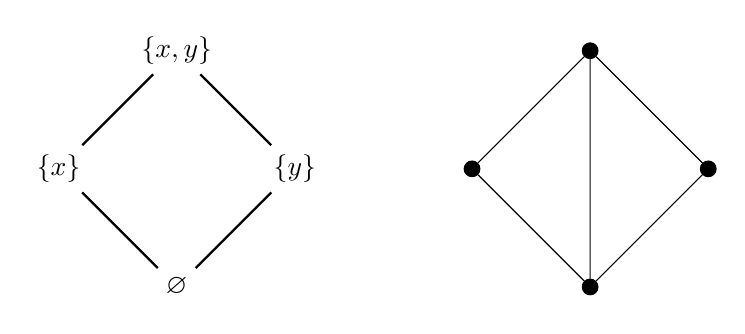
\begin{tikzpicture}[scale=1.5]

  % poset
  \draw (-1cm,0cm) node (v2) {$\{x\}$};
  \draw (1cm,0cm)  node (v3) { $\{y\}$ };
  \draw (0cm,-1cm) node (v4) {$\varnothing$};
  \draw (0cm,1cm)  node (v1) {$\{x,y\}$};

  \draw[thick]  (v1) edge (v2);
  \draw[thick]  (v3) edge (v1);
  \draw[thick]  (v3) edge (v4);
  \draw[thick]  (v2) edge (v4);

  % graph
  \node[draw,circle,inner sep=2pt,fill,label distance=1cm] (v1g) at (3.5,1) {};
  \node[draw,circle,inner sep=2pt,fill,label distance=1cm] (v2g) at (3.5,-1) {};
  \node[draw,circle,inner sep=2pt,fill,label distance=1cm] (v3g) at (4.5,0) {};
  \node[draw,circle,inner sep=2pt,fill,label distance=1cm] (v4g) at (2.5,0) {};
  \draw  (v1g) edge (v2g);
  \draw  (v1g) edge (v4g);
  \draw  (v4g) edge (v2g);
  \draw  (v1g) edge (v3g);
  \draw  (v3g) edge (v2g);

\end{tikzpicture}
\end{scaletikzpicturetowidth}

\caption{On the left, Hasse diagram of a poset of the power set of 2 elements ordered by inclusion.
On the right, the comparability graph of this poset.}
\label{fig:hasse}
\end{figure}

\subsubsection{Disks}

A disk graph $G$ is a graph that is an intersection graph of disks on the plane, when the size
of the disk is unitary, we talk about unit disk graphs. This class of graphs
is important for this thesis, as thin strip graphs are a sub-class of
unit disk graphs.

We will refer to the unit disk graph class as UDG and an example of a realization
can be found in the figure \ref{fig:udg}.

\paragraph{Induced forbidden subgraphs} The characterization of this class with respect to
its induced forbidden subgraphs has been studied \cite{atminasForbiddenInducedSubgraphs2016}.

\begin{theorem}[Atminas-Zamaraev]
  For every integer $k > 1$, $\overline{K_2 + C_{2k+1}}$ is a minimal induced subgraph of UDG.
\end{theorem}

\begin{theorem}[Atminas-Zamaraev]
  For every integer $k > 4$, $\overline{C_{2k}}$ is a minimal induced subgraph of UDG.
\end{theorem}

\begin{figure}
\centering

\begin{scaletikzpicturetowidth}{\textwidth}
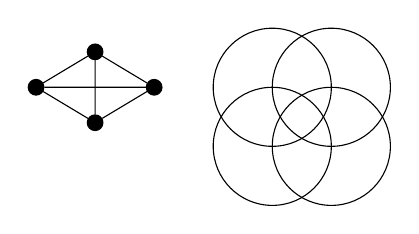
\begin{tikzpicture}[scale=1.5]

  \draw (-0.5,2.5) circle [radius=0.5];
  \draw (0,2.5) circle [radius=0.5];
  \draw (-0.5,2) circle [radius=0.5];
  \draw (0,2) circle [radius=0.5];


  \node[draw,circle,inner sep=2pt,fill,label distance=1cm] (v1) at (-2.5,2.5) {};

  \node[draw,circle,inner sep=2pt,fill,label distance=1cm] (v2) at (-2,2.2) {};
  \node[draw,circle,inner sep=2pt,fill,label distance=1cm] (v3) at (-2,2.8) {};
  \node[draw,circle,inner sep=2pt,fill,label distance=1cm] (v4) at (-1.5,2.5) {};

  \draw  (v3) edge (v2);
  \draw  (v4) edge (v1);
  \draw  (v3) edge (v1);
  \draw  (v4) edge (v2);
  \draw  (v3) edge (v4);
  \draw  (v1) edge (v2);

\end{tikzpicture}
\end{scaletikzpicturetowidth}

\caption{Realization of a UDG (Unit Disk Graph).}
\label{fig:udg}
\end{figure}

%\input{chap1/complexity}
%%% This is an example first chapter.  You should put chapter/appendix that you
%% write into a separate file, and add a line \include{yourfilename} to
%% main.tex, where `yourfilename.tex' is the name of the chapter/appendix file.
%% You can process specific files by typing their names in at the
%% \files=
%% prompt when you run the file main.tex through LaTeX.
\section{Geometry}
\label{sec:geom}

\begin{defn}
  $\text{dist}(a,b)$ denotes the distance between the points $a$ and $b$ and is calculated with:

  $$\text{dist}(a,b) = \sqrt{(a_x - b_x)^2 + (a_y - b_y)^2}$$
\end{defn}

The intersection of convex objects is a matter well studied for multiple
subjects. In our case, it is interesting to know some properties about
the intersection of disks, those ones being convex objects.

A set $S$ is convex if:
$$\forall p,q \in S\  \forall \lambda \in [0,1]: (1-\lambda)p + \lambda q \in S$$

\subsection{Stabbing}
A \textit{stabbing} is a point that traverses a set of intersecting objects. A lot of
research has been done \cite{schlipf2013stabbing} on the minimal amount of stabbings to
cover every object in a set. Stabbings can also be done with more complex structures
than points, in that case we are talking about \textit{coverings}.

\begin{theorem}[Helly]
  Given a set $Q$ of objects in $\mathbb{R}^d$, if for each subset of $Q$ of
  size $d+1$ their intersection is non empty, then $\bigcap_{q \in Q} \neq
  \varnothing$. \cite{Helly1923175}
\end{theorem}

\begin{theorem}
  The problem that for a set of $n$ disks whether there exists a regular n-gon
  whose vertices stab every disk of the set can be decided in $O(n^{10.5} / \sqrt{\log(n)})$ \cite{schlipf2013stabbing}
\end{theorem}

\subsection{Coin graphs}

Penny graphs can be defined as disk graphs where the disks can just touch each
other without overlapping. A famous theorem is derived from this class of graphs:
the circle packing theorem.

\begin{theorem}[Circle packing theorem]
  The circle packing theorem states that every simple connected planar graph
  $G$ is a penny graph. \cite{doi:10.1137/0406017}
\end{theorem}

\begin{corollary}
  Planar graphs $\subseteq$ disk graphs \cite{spinradEfficientGraphRepresentations2012}.
\end{corollary}

\begin{figure}
\centering
\includegraphics[width=1.0\textwidth]{res/circle_packing}
\caption{Circle packing of a planar graph. \cite{nachmiasPlanarMapsRandom2016}}
\label{fig:circle}
\end{figure}


\section{Graph theory}

A \emph{graph} is defined as a tuple $G = (V,E)$ where $V$ is the set of \emph{vertices} and $E$. When the the set of \emph{edges}, where $E = \binom{V}{2}$. If two vertices are share the same edge $e$ they are called \emph{adjacent} and also the \emph{endpoints} of $e$. A \emph{subgraph} $H = (V', E')$ of a graph $G$ is a graph such that $V' \subseteq V$ and $E' \subseteq E$. An \emph{induced subgraph} of a graph is a subgraph $H$ of a graph $G$ such that for every edge of $G$ is also in $H$ if its two endpoints are in $V'$. A \emph{clique} is a subgraph such that every vertex is adjacent to each other. A graph that is also a clique is called a \emph{complete graph} and it is denoted as $K_n$. A graph is \emph{bipartite} if there exist two disjoint subsets of the vertex set $A \cup B = V$ such that two vertices of the same subset are not adjacent. A \emph{complete bipartite graph} $K_{n,m}$ is a bipartite graph such that $v \in A$ and $w \in B$ implies $vw \in E$ where $n$ and $m$ are the size of each bipartition.

A \emph{path} $P_n = v_1\dots v_{n+1}$ of a graph is a sequence of $n$ vertices such that two consequent vertices are adjacent. A \emph{cycle} is a path $C_n = v_1\dots v_nv_{n+1}$ such that $v_1=v_{n+1}$. A graph is \emph{connected} if there exists a path between every pair of vertices. A \emph{chord} of a cycle $C_n$ with $n \geqslant 4$ is an edge that connects two non adjacent vertices of the cycle. A graph is \emph{chordal} if there is a chord in every cycle bigger than four.

\subsection{Intersection graphs}

\begin{figure}
\centering

\begin{scaletikzpicturetowidth}{\textwidth}
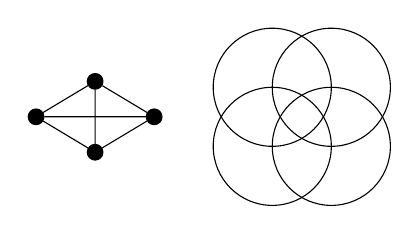
\begin{tikzpicture}[scale=1.5]

  \draw (-0.5,2.5) circle [radius=0.5];
  \draw (0,2.5) circle [radius=0.5];
  \draw (-0.5,2) circle [radius=0.5];
  \draw (0,2) circle [radius=0.5];


  \node[draw,circle,inner sep=2pt,fill,label distance=1cm] (v1) at (-2.5,2.25) {};

  \node[draw,circle,inner sep=2pt,fill,label distance=1cm] (v2) at (-2,1.95) {};
  \node[draw,circle,inner sep=2pt,fill,label distance=1cm] (v3) at (-2,2.55) {};
  \node[draw,circle,inner sep=2pt,fill,label distance=1cm] (v4) at (-1.5,2.25) {};

  \draw  (v3) edge (v2);
  \draw  (v4) edge (v1);
  \draw  (v3) edge (v1);
  \draw  (v4) edge (v2);
  \draw  (v3) edge (v4);
  \draw  (v1) edge (v2);

\end{tikzpicture}
\end{scaletikzpicturetowidth}

\caption{Realization of a UDG (unit disk graph).}
\label{fig:udg}
\end{figure}


An \emph{intersection graph} is a graph $G = (\zeta,E)$ of a collection of objects $\zeta$ is a graph such that $v,w \in \zeta$ and $v \cup w \neq \varnothing$ implies that $vw \in E$. An \emph{interval graph} is an intersection graph of intervals on the plane; when the size of the intervals is equal they are called \emph{unit interval graphs}. A \emph{unit disk graph} is an intersection graph of disks on a plane that have the same diameter - you can find an example in Figure \ref{fig:udg}.

\section{Order and set theory}

The \emph{powerset} $\powerset(S)$ of a set $S$ is the set of subsets of $S$. A \emph{partial order} is a binary relation $\leqslant$ over a set $A$ satisfying three axioms:

\begin{itemize}
  \item if $a \leqslant b$ and $b \leqslant a$ then $a = b$ (\emph{antisymmetry}).
  \item if $a \leqslant b$ and $b \leqslant c$ then $a \leqslant c$ (\emph{transitivity}).
  \item $a \leqslant a$ (\emph{reflexivity}).
\end{itemize}

\begin{figure}
\centering

\begin{scaletikzpicturetowidth}{\textwidth}
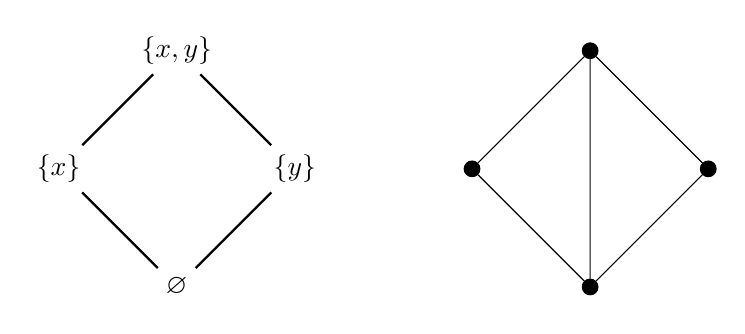
\begin{tikzpicture}[scale=1.5]

  % poset
  \draw (-1cm,0cm) node (v2) {$\{x\}$};
  \draw (1cm,0cm)  node (v3) { $\{y\}$ };
  \draw (0cm,-1cm) node (v4) {$\varnothing$};
  \draw (0cm,1cm)  node (v1) {$\{x,y\}$};

  \draw[thick]  (v1) edge (v2);
  \draw[thick]  (v3) edge (v1);
  \draw[thick]  (v3) edge (v4);
  \draw[thick]  (v2) edge (v4);

  % graph
  \node[draw,circle,inner sep=2pt,fill,label distance=1cm] (v1g) at (3.5,1) {};
  \node[draw,circle,inner sep=2pt,fill,label distance=1cm] (v2g) at (3.5,-1) {};
  \node[draw,circle,inner sep=2pt,fill,label distance=1cm] (v3g) at (4.5,0) {};
  \node[draw,circle,inner sep=2pt,fill,label distance=1cm] (v4g) at (2.5,0) {};
  \draw  (v1g) edge (v2g);
  \draw  (v1g) edge (v4g);
  \draw  (v4g) edge (v2g);
  \draw  (v1g) edge (v3g);
  \draw  (v3g) edge (v2g);

\end{tikzpicture}
\end{scaletikzpicturetowidth}

\caption{On the left, Hasse diagram of a poset of the power set of 2 elements ordered by inclusion.
On the right, the comparability graph of this poset.}
\label{fig:hasse}
\end{figure}

In the other side, a \emph{total order} is a partial order where the reflexivity order is replaced by the \emph{connexity} property -- $a \leq b\ \text{or}\  b \leq a$. A \emph{partially ordered set} (or \emph{poset}) $(S,\leqslant)$ is a set such that the elements of $S$ are partially ordered by the relation $\leqslant$. A good way to represent a poset is the \emph{Hasse diagram} (figure \ref{fig:hasse}).

\subsection{Comparability graphs}

A \emph{spanning order} $(V,<)$ on a graph $G = (V,E)$ is a total order on $V$ such that for any three vertices $u < v < w$:

  $$uw \in E \to uv \in E\ \text{or}\ vw \in E$$

The class of comparability graphs are built on the ideas of order theory. A graph $G$ is a \emph{comparability graph} if there exists a partial order $\leqslant$ such that $uv \in E \Leftrightarrow v \leqslant w\  \text{or}\  w \leqslant v$.

\section{Geometry}

\chapter{Background}
\label{chap:background}

In this chapter we review some definitions and notations of the background knowledge of this thesis. We limit ourselves to the basic notations used during the work. Nevertheless, the bibliography of each subject will be referenced for further details about the topic.

%\todo{Text about background intro}

%%% This is an example first chapter.  You should put chapter/appendix that you
%% write into a separate file, and add a line \include{yourfilename} to
%% main.tex, where `yourfilename.tex' is the name of the chapter/appendix file.
%% You can process specific files by typing their names in at the
%% \files=
%% prompt when you run the file main.tex through LaTeX.
\section{Graphs and intersections}
\label{sec:graphs}


\subsection{Graphs}

A graph $G$ is defined as $G = (V,E)$, where $V$ is the set of vertices and $E$ the set of
edges, where $E \subseteq \binom{V}{2}$. The vertices $v,w \in V$ such that $e = vw \in E$
links are called the \textit{endpoints} of $e$.

\begin{defn}
  An embedding of a graph $G$ into a surface $\Sigma$ is a mapping of $G$ in
  $\Sigma$ where the vertices correspond to distinct points and the edges
  correspond to simple arcs connecting the images of their endpoints.
  \cite{goyalGraphEmbeddingTechniques2017}.
\end{defn}

A graph $G$ is planar if there is an embedding of this graph that does not have
any crossing between the edges.

\begin{defn}
  Let $G = (V,E)$ and $S \subset V$, an induced subgraph is a graph $H$ of $G$ whose
  vertex set is $S$ and its edge set $F = \{vw : v,w \in S, vw \in E\}$.
\end{defn}

\begin{defn}
  Let $G = (V,E)$ its complement graph $\overline{G}$ is the graph such that its edge set
  is defined as: $\{vw: v,w\in V, vw\notin E\}$.
\end{defn}

\begin{defn}
  $H$ is called a \textit{minor} of $G$ if $H$ can be constructed by deleting edges and vertices,
  or contracting edges.
\end{defn}

\begin{theorem}[Kuratowski]
  \label{theo:kura}
  A graph $G$ is planar if and only if it does not contain $K_5$ or $K_{3,3}$ as a minor or
  a induced subgraph.
\end{theorem}

\begin{defn}
  A path $P_n$ in a graph $G$ is a sequence of vertices $v_1v_2v_3\dots v_n$ such
  that $v_iv_{i+1} \in E$.
\end{defn}

\begin{defn}
  A cycle $C_n$ in a graph $G = (V,E)$ is a path $v_1\dots v_n$ such that $v_1 = v_n$.
\end{defn}

\begin{defn}
  A chord of a cycle $C_n$ with $n \geq 4 $ is an edge that connects two non consecutive vertices
  of $C_n$.
\end{defn}

\begin{defn}
  A triangular chord of a cycle is a chord that will create a new triangle ($C_3$).
\end{defn}


\begin{defn}
  A graph $G = (V,E)$ is complete if every pair of distinct $v_1,v_2 \in V$ are
  adjacent. This is denoted $K_n$ with $n$ the size of the graph. If $G$ is an
  induced graph of $H$ then $G$ is a clique of $H$.
\end{defn}

\begin{defn}
  A graph $G$ is bipartite if there exist two disjoint subsets $A,B \subset V$ such
  that $A\cup B = V$ and each edge $e\in E$ has an endpoint on $A$ and the
  another on $B$.
\end{defn}

\begin{defn}
  A bipartite graph $G$ with bipartitions $A$ and $B$ is complete bipartite if
  every pair of vertices $v\in A, w\in B$ are adjacent. It is denoted as $K_{n,m}$,
  being $n$ and $m$ the size of each bipartition.
\end{defn}

Some graphs can be characterized with properties. A property of a graph is a property that
is preserved under all its isomophisms. These properties are called \textit{hereditary} if they
are also preserved under all its induced subgraphs; they are called \textit{minor-hereditary} if they are
also preserved under its minors (e.g. Kuratowski's planar graph characterization [\ref{theo:kura}]).

\begin{defn}
  An forbidden induced subgraph (minor) of a graph class $X$ is a graph such that if it is the induced
  subgraph (minor) of a graph $G$, we know that $G \notin X$.
\end{defn}

The coloration of a graph is a color assignment to each vertex such that the color
of the two endpoints of every edge of the graph is different.

\begin{defn}
  The chromatic number of a graph $\chi(G)$ is the smallest number of colors needed to
  have an acceptable coloration of $G$.
\end{defn}

\begin{defn}
  The clique number of a graph $\omega(G)$ is the size of the biggest clique of $G$. We
  can observe that for every graph: $\chi(G) \geq \omega(G)$.
\end{defn}

\begin{defn}
  A perfect graph is a graph that respects this condition for every induced subgraph:
  $$ \omega(G) = \chi(G)$$
\end{defn}

\begin{theorem}[Lovasz]
  $G$ is perfect if and only if $\overline{G}$ is perfect.
\end{theorem}

\subsection{Intersection graphs}

\begin{defn}
The \textit{intersection graph} of a collection $\zeta$ of objects is the graph
$(\zeta,E)$ such that $c_1c_2\in E \Leftrightarrow c_1 \cap c_2 \neq \varnothing$.
\end{defn}

An intersection can be seen as a relationship between two objects. In this thesis, it will be important to define these relations more formally to characterize intersection graphs.

\begin{defn}
  A partial order is a binary relation $\leq$ over a set $A$ satisfying these axioms:
  \begin{itemize}
    \item if $a \leq b$ and $b \leq a$ then $a = b$ (antisymmetry).
    \item if $a \leq b$ and $b \leq c$ then $a \leq c$ (transitivity).
    \item $a \leq a$ (reflexivity).
  \end{itemize}
\end{defn}

\begin{defn}
  A total order is a partial order where the reflexivity order is replaced by the connex property:
  $$a \leq b\ \text{or}\  b \leq a$$
\end{defn}

\begin{defn}
   A partially ordered set or poset  $(S,\leq)$ where $S$ a set and $\leq$ a partial
   order on $S$.
\end{defn}

\begin{defn}
  A spanning order $(V,<)$ of a graph $G = (V,E)$ is a total order on $V$ such that for any three vertices $u < v < w$:

  $$uw \in E \to uv \in E\ \text{or}\ vw \in E$$
\end{defn}


\begin{defn}
  A graph $G = (V,E)$ is a comparibility graph if there exists a partial order
  $\leq$ such that $vw \in E \Leftrightarrow v \leq w$ or $w \leq v$.
  Equivalently, $G$ is a comparability graph if it is the comparability graph of
  a poset. For example, the Hasse diagram (figure \ref{fig:hasse}) is a
  comparability graph where the relation is inclusion.
\end{defn}

\begin{defn}
  A graph $G = (V,E)$ is a co-comparability graph if its complement is a comparability graph.
\end{defn}

There are multiple characterizations for the co-comparability graph class; we will see one that uses a poset to characterize it:

\begin{theorem}[Damaschke \cite{damaschkeDistancesCocomparabilityGraphs1992}]
  \label{theo:spanning}
  A graph $G$ is a co-comparability graph if and only if it has a spanning order.
\end{theorem}


\begin{figure}
\centering

\begin{scaletikzpicturetowidth}{\textwidth}
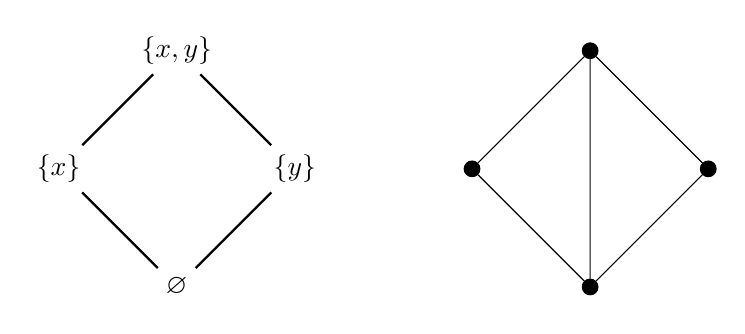
\begin{tikzpicture}[scale=1.5]

  % poset
  \draw (-1cm,0cm) node (v2) {$\{x\}$};
  \draw (1cm,0cm)  node (v3) { $\{y\}$ };
  \draw (0cm,-1cm) node (v4) {$\varnothing$};
  \draw (0cm,1cm)  node (v1) {$\{x,y\}$};

  \draw[thick]  (v1) edge (v2);
  \draw[thick]  (v3) edge (v1);
  \draw[thick]  (v3) edge (v4);
  \draw[thick]  (v2) edge (v4);

  % graph
  \node[draw,circle,inner sep=2pt,fill,label distance=1cm] (v1g) at (3.5,1) {};
  \node[draw,circle,inner sep=2pt,fill,label distance=1cm] (v2g) at (3.5,-1) {};
  \node[draw,circle,inner sep=2pt,fill,label distance=1cm] (v3g) at (4.5,0) {};
  \node[draw,circle,inner sep=2pt,fill,label distance=1cm] (v4g) at (2.5,0) {};
  \draw  (v1g) edge (v2g);
  \draw  (v1g) edge (v4g);
  \draw  (v4g) edge (v2g);
  \draw  (v1g) edge (v3g);
  \draw  (v3g) edge (v2g);

\end{tikzpicture}
\end{scaletikzpicturetowidth}

\caption{On the left, Hasse diagram of a poset of the power set of 2 elements ordered by inclusion.
On the right, the comparability graph of this poset.}
\label{fig:hasse}
\end{figure}

\subsubsection{Disks}

A disk graph $G$ is a graph that is an intersection graph of disks on the plane, when the size
of the disk is unitary, we talk about unit disk graphs. This class of graphs
is important for this thesis, as thin strip graphs are a sub-class of
unit disk graphs.

We will refer to the unit disk graph class as UDG and an example of a realization
can be found in the figure \ref{fig:udg}.

\paragraph{Induced forbidden subgraphs} The characterization of this class with respect to
its induced forbidden subgraphs has been studied \cite{atminasForbiddenInducedSubgraphs2016}.

\begin{theorem}[Atminas-Zamaraev]
  For every integer $k > 1$, $\overline{K_2 + C_{2k+1}}$ is a minimal induced subgraph of UDG.
\end{theorem}

\begin{theorem}[Atminas-Zamaraev]
  For every integer $k > 4$, $\overline{C_{2k}}$ is a minimal induced subgraph of UDG.
\end{theorem}

\begin{figure}
\centering

\begin{scaletikzpicturetowidth}{\textwidth}
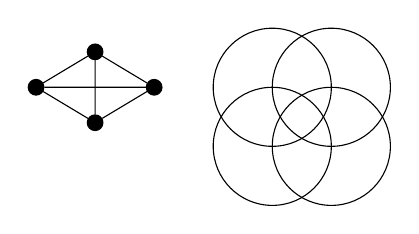
\begin{tikzpicture}[scale=1.5]

  \draw (-0.5,2.5) circle [radius=0.5];
  \draw (0,2.5) circle [radius=0.5];
  \draw (-0.5,2) circle [radius=0.5];
  \draw (0,2) circle [radius=0.5];


  \node[draw,circle,inner sep=2pt,fill,label distance=1cm] (v1) at (-2.5,2.5) {};

  \node[draw,circle,inner sep=2pt,fill,label distance=1cm] (v2) at (-2,2.2) {};
  \node[draw,circle,inner sep=2pt,fill,label distance=1cm] (v3) at (-2,2.8) {};
  \node[draw,circle,inner sep=2pt,fill,label distance=1cm] (v4) at (-1.5,2.5) {};

  \draw  (v3) edge (v2);
  \draw  (v4) edge (v1);
  \draw  (v3) edge (v1);
  \draw  (v4) edge (v2);
  \draw  (v3) edge (v4);
  \draw  (v1) edge (v2);

\end{tikzpicture}
\end{scaletikzpicturetowidth}

\caption{Realization of a UDG (Unit Disk Graph).}
\label{fig:udg}
\end{figure}

%\input{chap1/complexity}
%%% This is an example first chapter.  You should put chapter/appendix that you
%% write into a separate file, and add a line \include{yourfilename} to
%% main.tex, where `yourfilename.tex' is the name of the chapter/appendix file.
%% You can process specific files by typing their names in at the
%% \files=
%% prompt when you run the file main.tex through LaTeX.
\section{Geometry}
\label{sec:geom}

\begin{defn}
  $\text{dist}(a,b)$ denotes the distance between the points $a$ and $b$ and is calculated with:

  $$\text{dist}(a,b) = \sqrt{(a_x - b_x)^2 + (a_y - b_y)^2}$$
\end{defn}

The intersection of convex objects is a matter well studied for multiple
subjects. In our case, it is interesting to know some properties about
the intersection of disks, those ones being convex objects.

A set $S$ is convex if:
$$\forall p,q \in S\  \forall \lambda \in [0,1]: (1-\lambda)p + \lambda q \in S$$

\subsection{Stabbing}
A \textit{stabbing} is a point that traverses a set of intersecting objects. A lot of
research has been done \cite{schlipf2013stabbing} on the minimal amount of stabbings to
cover every object in a set. Stabbings can also be done with more complex structures
than points, in that case we are talking about \textit{coverings}.

\begin{theorem}[Helly]
  Given a set $Q$ of objects in $\mathbb{R}^d$, if for each subset of $Q$ of
  size $d+1$ their intersection is non empty, then $\bigcap_{q \in Q} \neq
  \varnothing$. \cite{Helly1923175}
\end{theorem}

\begin{theorem}
  The problem that for a set of $n$ disks whether there exists a regular n-gon
  whose vertices stab every disk of the set can be decided in $O(n^{10.5} / \sqrt{\log(n)})$ \cite{schlipf2013stabbing}
\end{theorem}

\subsection{Coin graphs}

Penny graphs can be defined as disk graphs where the disks can just touch each
other without overlapping. A famous theorem is derived from this class of graphs:
the circle packing theorem.

\begin{theorem}[Circle packing theorem]
  The circle packing theorem states that every simple connected planar graph
  $G$ is a penny graph. \cite{doi:10.1137/0406017}
\end{theorem}

\begin{corollary}
  Planar graphs $\subseteq$ disk graphs \cite{spinradEfficientGraphRepresentations2012}.
\end{corollary}

\begin{figure}
\centering
\includegraphics[width=1.0\textwidth]{res/circle_packing}
\caption{Circle packing of a planar graph. \cite{nachmiasPlanarMapsRandom2016}}
\label{fig:circle}
\end{figure}


\section{Graph theory}

A \emph{graph} is defined as a tuple $G = (V,E)$ where $V$ is the set of \emph{vertices} and $E$. When the the set of \emph{edges}, where $E = \binom{V}{2}$. If two vertices are share the same edge $e$ they are called \emph{adjacent} and also the \emph{endpoints} of $e$. A \emph{subgraph} $H = (V', E')$ of a graph $G$ is a graph such that $V' \subseteq V$ and $E' \subseteq E$. An \emph{induced subgraph} of a graph is a subgraph $H$ of a graph $G$ such that for every edge of $G$ is also in $H$ if its two endpoints are in $V'$. A \emph{clique} is a subgraph such that every vertex is adjacent to each other. A graph that is also a clique is called a \emph{complete graph} and it is denoted as $K_n$. A graph is \emph{bipartite} if there exist two disjoint subsets of the vertex set $A \cup B = V$ such that two vertices of the same subset are not adjacent. A \emph{complete bipartite graph} $K_{n,m}$ is a bipartite graph such that $v \in A$ and $w \in B$ implies $vw \in E$ where $n$ and $m$ are the size of each bipartition.

A \emph{path} $P_n = v_1\dots v_{n+1}$ of a graph is a sequence of $n$ vertices such that two consequent vertices are adjacent. A \emph{cycle} is a path $C_n = v_1\dots v_nv_{n+1}$ such that $v_1=v_{n+1}$. A graph is \emph{connected} if there exists a path between every pair of vertices. A \emph{chord} of a cycle $C_n$ with $n \geqslant 4$ is an edge that connects two non adjacent vertices of the cycle. A graph is \emph{chordal} if there is a chord in every cycle bigger than four.

\subsection{Intersection graphs}

\begin{figure}
\centering

\begin{scaletikzpicturetowidth}{\textwidth}
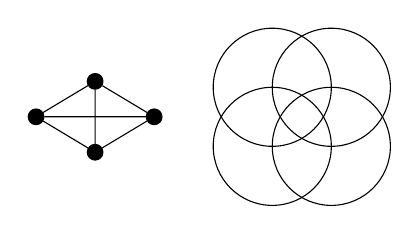
\begin{tikzpicture}[scale=1.5]

  \draw (-0.5,2.5) circle [radius=0.5];
  \draw (0,2.5) circle [radius=0.5];
  \draw (-0.5,2) circle [radius=0.5];
  \draw (0,2) circle [radius=0.5];


  \node[draw,circle,inner sep=2pt,fill,label distance=1cm] (v1) at (-2.5,2.25) {};

  \node[draw,circle,inner sep=2pt,fill,label distance=1cm] (v2) at (-2,1.95) {};
  \node[draw,circle,inner sep=2pt,fill,label distance=1cm] (v3) at (-2,2.55) {};
  \node[draw,circle,inner sep=2pt,fill,label distance=1cm] (v4) at (-1.5,2.25) {};

  \draw  (v3) edge (v2);
  \draw  (v4) edge (v1);
  \draw  (v3) edge (v1);
  \draw  (v4) edge (v2);
  \draw  (v3) edge (v4);
  \draw  (v1) edge (v2);

\end{tikzpicture}
\end{scaletikzpicturetowidth}

\caption{Realization of a UDG (unit disk graph).}
\label{fig:udg}
\end{figure}


An \emph{intersection graph} is a graph $G = (\zeta,E)$ of a collection of objects $\zeta$ is a graph such that $v,w \in \zeta$ and $v \cup w \neq \varnothing$ implies that $vw \in E$. An \emph{interval graph} is an intersection graph of intervals on the plane; when the size of the intervals is equal they are called \emph{unit interval graphs}. A \emph{unit disk graph} is an intersection graph of disks on a plane that have the same diameter - you can find an example in Figure \ref{fig:udg}.

\section{Order and set theory}

The \emph{powerset} $\powerset(S)$ of a set $S$ is the set of subsets of $S$. A \emph{partial order} is a binary relation $\leqslant$ over a set $A$ satisfying three axioms:

\begin{itemize}
  \item if $a \leqslant b$ and $b \leqslant a$ then $a = b$ (\emph{antisymmetry}).
  \item if $a \leqslant b$ and $b \leqslant c$ then $a \leqslant c$ (\emph{transitivity}).
  \item $a \leqslant a$ (\emph{reflexivity}).
\end{itemize}

\begin{figure}
\centering

\begin{scaletikzpicturetowidth}{\textwidth}
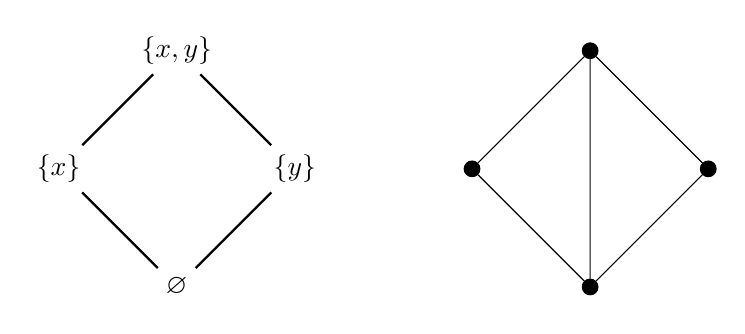
\begin{tikzpicture}[scale=1.5]

  % poset
  \draw (-1cm,0cm) node (v2) {$\{x\}$};
  \draw (1cm,0cm)  node (v3) { $\{y\}$ };
  \draw (0cm,-1cm) node (v4) {$\varnothing$};
  \draw (0cm,1cm)  node (v1) {$\{x,y\}$};

  \draw[thick]  (v1) edge (v2);
  \draw[thick]  (v3) edge (v1);
  \draw[thick]  (v3) edge (v4);
  \draw[thick]  (v2) edge (v4);

  % graph
  \node[draw,circle,inner sep=2pt,fill,label distance=1cm] (v1g) at (3.5,1) {};
  \node[draw,circle,inner sep=2pt,fill,label distance=1cm] (v2g) at (3.5,-1) {};
  \node[draw,circle,inner sep=2pt,fill,label distance=1cm] (v3g) at (4.5,0) {};
  \node[draw,circle,inner sep=2pt,fill,label distance=1cm] (v4g) at (2.5,0) {};
  \draw  (v1g) edge (v2g);
  \draw  (v1g) edge (v4g);
  \draw  (v4g) edge (v2g);
  \draw  (v1g) edge (v3g);
  \draw  (v3g) edge (v2g);

\end{tikzpicture}
\end{scaletikzpicturetowidth}

\caption{On the left, Hasse diagram of a poset of the power set of 2 elements ordered by inclusion.
On the right, the comparability graph of this poset.}
\label{fig:hasse}
\end{figure}

In the other side, a \emph{total order} is a partial order where the reflexivity order is replaced by the \emph{connexity} property -- $a \leq b\ \text{or}\  b \leq a$. A \emph{partially ordered set} (or \emph{poset}) $(S,\leqslant)$ is a set such that the elements of $S$ are partially ordered by the relation $\leqslant$. A good way to represent a poset is the \emph{Hasse diagram} (figure \ref{fig:hasse}).

\subsection{Comparability graphs}

A \emph{spanning order} $(V,<)$ on a graph $G = (V,E)$ is a total order on $V$ such that for any three vertices $u < v < w$:

  $$uw \in E \to uv \in E\ \text{or}\ vw \in E$$

The class of comparability graphs are built on the ideas of order theory. A graph $G$ is a \emph{comparability graph} if there exists a partial order $\leqslant$ such that $uv \in E \Leftrightarrow v \leqslant w\  \text{or}\  w \leqslant v$.

\section{Geometry}


%% CHAPTERS %%


\chapter{Background}
\label{chap:background}

In this chapter we review some definitions and notations of the background knowledge of this thesis. We limit ourselves to the basic notations used during the work. Nevertheless, the bibliography of each subject will be referenced for further details about the topic.

%\todo{Text about background intro}

%%% This is an example first chapter.  You should put chapter/appendix that you
%% write into a separate file, and add a line \include{yourfilename} to
%% main.tex, where `yourfilename.tex' is the name of the chapter/appendix file.
%% You can process specific files by typing their names in at the
%% \files=
%% prompt when you run the file main.tex through LaTeX.
\section{Graphs and intersections}
\label{sec:graphs}


\subsection{Graphs}

A graph $G$ is defined as $G = (V,E)$, where $V$ is the set of vertices and $E$ the set of
edges, where $E \subseteq \binom{V}{2}$. The vertices $v,w \in V$ such that $e = vw \in E$
links are called the \textit{endpoints} of $e$.

\begin{defn}
  An embedding of a graph $G$ into a surface $\Sigma$ is a mapping of $G$ in
  $\Sigma$ where the vertices correspond to distinct points and the edges
  correspond to simple arcs connecting the images of their endpoints.
  \cite{goyalGraphEmbeddingTechniques2017}.
\end{defn}

A graph $G$ is planar if there is an embedding of this graph that does not have
any crossing between the edges.

\begin{defn}
  Let $G = (V,E)$ and $S \subset V$, an induced subgraph is a graph $H$ of $G$ whose
  vertex set is $S$ and its edge set $F = \{vw : v,w \in S, vw \in E\}$.
\end{defn}

\begin{defn}
  Let $G = (V,E)$ its complement graph $\overline{G}$ is the graph such that its edge set
  is defined as: $\{vw: v,w\in V, vw\notin E\}$.
\end{defn}

\begin{defn}
  $H$ is called a \textit{minor} of $G$ if $H$ can be constructed by deleting edges and vertices,
  or contracting edges.
\end{defn}

\begin{theorem}[Kuratowski]
  \label{theo:kura}
  A graph $G$ is planar if and only if it does not contain $K_5$ or $K_{3,3}$ as a minor or
  a induced subgraph.
\end{theorem}

\begin{defn}
  A path $P_n$ in a graph $G$ is a sequence of vertices $v_1v_2v_3\dots v_n$ such
  that $v_iv_{i+1} \in E$.
\end{defn}

\begin{defn}
  A cycle $C_n$ in a graph $G = (V,E)$ is a path $v_1\dots v_n$ such that $v_1 = v_n$.
\end{defn}

\begin{defn}
  A chord of a cycle $C_n$ with $n \geq 4 $ is an edge that connects two non consecutive vertices
  of $C_n$.
\end{defn}

\begin{defn}
  A triangular chord of a cycle is a chord that will create a new triangle ($C_3$).
\end{defn}


\begin{defn}
  A graph $G = (V,E)$ is complete if every pair of distinct $v_1,v_2 \in V$ are
  adjacent. This is denoted $K_n$ with $n$ the size of the graph. If $G$ is an
  induced graph of $H$ then $G$ is a clique of $H$.
\end{defn}

\begin{defn}
  A graph $G$ is bipartite if there exist two disjoint subsets $A,B \subset V$ such
  that $A\cup B = V$ and each edge $e\in E$ has an endpoint on $A$ and the
  another on $B$.
\end{defn}

\begin{defn}
  A bipartite graph $G$ with bipartitions $A$ and $B$ is complete bipartite if
  every pair of vertices $v\in A, w\in B$ are adjacent. It is denoted as $K_{n,m}$,
  being $n$ and $m$ the size of each bipartition.
\end{defn}

Some graphs can be characterized with properties. A property of a graph is a property that
is preserved under all its isomophisms. These properties are called \textit{hereditary} if they
are also preserved under all its induced subgraphs; they are called \textit{minor-hereditary} if they are
also preserved under its minors (e.g. Kuratowski's planar graph characterization [\ref{theo:kura}]).

\begin{defn}
  An forbidden induced subgraph (minor) of a graph class $X$ is a graph such that if it is the induced
  subgraph (minor) of a graph $G$, we know that $G \notin X$.
\end{defn}

The coloration of a graph is a color assignment to each vertex such that the color
of the two endpoints of every edge of the graph is different.

\begin{defn}
  The chromatic number of a graph $\chi(G)$ is the smallest number of colors needed to
  have an acceptable coloration of $G$.
\end{defn}

\begin{defn}
  The clique number of a graph $\omega(G)$ is the size of the biggest clique of $G$. We
  can observe that for every graph: $\chi(G) \geq \omega(G)$.
\end{defn}

\begin{defn}
  A perfect graph is a graph that respects this condition for every induced subgraph:
  $$ \omega(G) = \chi(G)$$
\end{defn}

\begin{theorem}[Lovasz]
  $G$ is perfect if and only if $\overline{G}$ is perfect.
\end{theorem}

\subsection{Intersection graphs}

\begin{defn}
The \textit{intersection graph} of a collection $\zeta$ of objects is the graph
$(\zeta,E)$ such that $c_1c_2\in E \Leftrightarrow c_1 \cap c_2 \neq \varnothing$.
\end{defn}

An intersection can be seen as a relationship between two objects. In this thesis, it will be important to define these relations more formally to characterize intersection graphs.

\begin{defn}
  A partial order is a binary relation $\leq$ over a set $A$ satisfying these axioms:
  \begin{itemize}
    \item if $a \leq b$ and $b \leq a$ then $a = b$ (antisymmetry).
    \item if $a \leq b$ and $b \leq c$ then $a \leq c$ (transitivity).
    \item $a \leq a$ (reflexivity).
  \end{itemize}
\end{defn}

\begin{defn}
  A total order is a partial order where the reflexivity order is replaced by the connex property:
  $$a \leq b\ \text{or}\  b \leq a$$
\end{defn}

\begin{defn}
   A partially ordered set or poset  $(S,\leq)$ where $S$ a set and $\leq$ a partial
   order on $S$.
\end{defn}

\begin{defn}
  A spanning order $(V,<)$ of a graph $G = (V,E)$ is a total order on $V$ such that for any three vertices $u < v < w$:

  $$uw \in E \to uv \in E\ \text{or}\ vw \in E$$
\end{defn}


\begin{defn}
  A graph $G = (V,E)$ is a comparibility graph if there exists a partial order
  $\leq$ such that $vw \in E \Leftrightarrow v \leq w$ or $w \leq v$.
  Equivalently, $G$ is a comparability graph if it is the comparability graph of
  a poset. For example, the Hasse diagram (figure \ref{fig:hasse}) is a
  comparability graph where the relation is inclusion.
\end{defn}

\begin{defn}
  A graph $G = (V,E)$ is a co-comparability graph if its complement is a comparability graph.
\end{defn}

There are multiple characterizations for the co-comparability graph class; we will see one that uses a poset to characterize it:

\begin{theorem}[Damaschke \cite{damaschkeDistancesCocomparabilityGraphs1992}]
  \label{theo:spanning}
  A graph $G$ is a co-comparability graph if and only if it has a spanning order.
\end{theorem}


\begin{figure}
\centering

\begin{scaletikzpicturetowidth}{\textwidth}
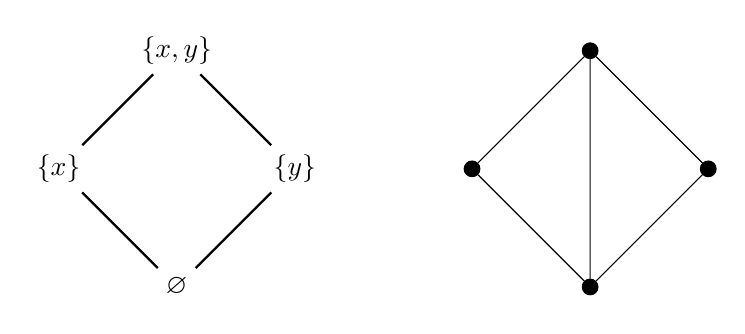
\begin{tikzpicture}[scale=1.5]

  % poset
  \draw (-1cm,0cm) node (v2) {$\{x\}$};
  \draw (1cm,0cm)  node (v3) { $\{y\}$ };
  \draw (0cm,-1cm) node (v4) {$\varnothing$};
  \draw (0cm,1cm)  node (v1) {$\{x,y\}$};

  \draw[thick]  (v1) edge (v2);
  \draw[thick]  (v3) edge (v1);
  \draw[thick]  (v3) edge (v4);
  \draw[thick]  (v2) edge (v4);

  % graph
  \node[draw,circle,inner sep=2pt,fill,label distance=1cm] (v1g) at (3.5,1) {};
  \node[draw,circle,inner sep=2pt,fill,label distance=1cm] (v2g) at (3.5,-1) {};
  \node[draw,circle,inner sep=2pt,fill,label distance=1cm] (v3g) at (4.5,0) {};
  \node[draw,circle,inner sep=2pt,fill,label distance=1cm] (v4g) at (2.5,0) {};
  \draw  (v1g) edge (v2g);
  \draw  (v1g) edge (v4g);
  \draw  (v4g) edge (v2g);
  \draw  (v1g) edge (v3g);
  \draw  (v3g) edge (v2g);

\end{tikzpicture}
\end{scaletikzpicturetowidth}

\caption{On the left, Hasse diagram of a poset of the power set of 2 elements ordered by inclusion.
On the right, the comparability graph of this poset.}
\label{fig:hasse}
\end{figure}

\subsubsection{Disks}

A disk graph $G$ is a graph that is an intersection graph of disks on the plane, when the size
of the disk is unitary, we talk about unit disk graphs. This class of graphs
is important for this thesis, as thin strip graphs are a sub-class of
unit disk graphs.

We will refer to the unit disk graph class as UDG and an example of a realization
can be found in the figure \ref{fig:udg}.

\paragraph{Induced forbidden subgraphs} The characterization of this class with respect to
its induced forbidden subgraphs has been studied \cite{atminasForbiddenInducedSubgraphs2016}.

\begin{theorem}[Atminas-Zamaraev]
  For every integer $k > 1$, $\overline{K_2 + C_{2k+1}}$ is a minimal induced subgraph of UDG.
\end{theorem}

\begin{theorem}[Atminas-Zamaraev]
  For every integer $k > 4$, $\overline{C_{2k}}$ is a minimal induced subgraph of UDG.
\end{theorem}

\begin{figure}
\centering

\begin{scaletikzpicturetowidth}{\textwidth}
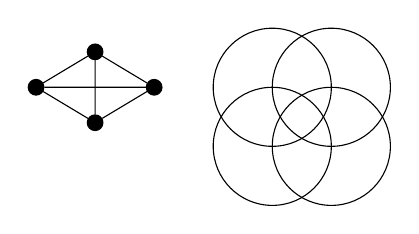
\begin{tikzpicture}[scale=1.5]

  \draw (-0.5,2.5) circle [radius=0.5];
  \draw (0,2.5) circle [radius=0.5];
  \draw (-0.5,2) circle [radius=0.5];
  \draw (0,2) circle [radius=0.5];


  \node[draw,circle,inner sep=2pt,fill,label distance=1cm] (v1) at (-2.5,2.5) {};

  \node[draw,circle,inner sep=2pt,fill,label distance=1cm] (v2) at (-2,2.2) {};
  \node[draw,circle,inner sep=2pt,fill,label distance=1cm] (v3) at (-2,2.8) {};
  \node[draw,circle,inner sep=2pt,fill,label distance=1cm] (v4) at (-1.5,2.5) {};

  \draw  (v3) edge (v2);
  \draw  (v4) edge (v1);
  \draw  (v3) edge (v1);
  \draw  (v4) edge (v2);
  \draw  (v3) edge (v4);
  \draw  (v1) edge (v2);

\end{tikzpicture}
\end{scaletikzpicturetowidth}

\caption{Realization of a UDG (Unit Disk Graph).}
\label{fig:udg}
\end{figure}

%\input{chap1/complexity}
%%% This is an example first chapter.  You should put chapter/appendix that you
%% write into a separate file, and add a line \include{yourfilename} to
%% main.tex, where `yourfilename.tex' is the name of the chapter/appendix file.
%% You can process specific files by typing their names in at the
%% \files=
%% prompt when you run the file main.tex through LaTeX.
\section{Geometry}
\label{sec:geom}

\begin{defn}
  $\text{dist}(a,b)$ denotes the distance between the points $a$ and $b$ and is calculated with:

  $$\text{dist}(a,b) = \sqrt{(a_x - b_x)^2 + (a_y - b_y)^2}$$
\end{defn}

The intersection of convex objects is a matter well studied for multiple
subjects. In our case, it is interesting to know some properties about
the intersection of disks, those ones being convex objects.

A set $S$ is convex if:
$$\forall p,q \in S\  \forall \lambda \in [0,1]: (1-\lambda)p + \lambda q \in S$$

\subsection{Stabbing}
A \textit{stabbing} is a point that traverses a set of intersecting objects. A lot of
research has been done \cite{schlipf2013stabbing} on the minimal amount of stabbings to
cover every object in a set. Stabbings can also be done with more complex structures
than points, in that case we are talking about \textit{coverings}.

\begin{theorem}[Helly]
  Given a set $Q$ of objects in $\mathbb{R}^d$, if for each subset of $Q$ of
  size $d+1$ their intersection is non empty, then $\bigcap_{q \in Q} \neq
  \varnothing$. \cite{Helly1923175}
\end{theorem}

\begin{theorem}
  The problem that for a set of $n$ disks whether there exists a regular n-gon
  whose vertices stab every disk of the set can be decided in $O(n^{10.5} / \sqrt{\log(n)})$ \cite{schlipf2013stabbing}
\end{theorem}

\subsection{Coin graphs}

Penny graphs can be defined as disk graphs where the disks can just touch each
other without overlapping. A famous theorem is derived from this class of graphs:
the circle packing theorem.

\begin{theorem}[Circle packing theorem]
  The circle packing theorem states that every simple connected planar graph
  $G$ is a penny graph. \cite{doi:10.1137/0406017}
\end{theorem}

\begin{corollary}
  Planar graphs $\subseteq$ disk graphs \cite{spinradEfficientGraphRepresentations2012}.
\end{corollary}

\begin{figure}
\centering
\includegraphics[width=1.0\textwidth]{res/circle_packing}
\caption{Circle packing of a planar graph. \cite{nachmiasPlanarMapsRandom2016}}
\label{fig:circle}
\end{figure}


\section{Graph theory}

A \emph{graph} is defined as a tuple $G = (V,E)$ where $V$ is the set of \emph{vertices} and $E$. When the the set of \emph{edges}, where $E = \binom{V}{2}$. If two vertices are share the same edge $e$ they are called \emph{adjacent} and also the \emph{endpoints} of $e$. A \emph{subgraph} $H = (V', E')$ of a graph $G$ is a graph such that $V' \subseteq V$ and $E' \subseteq E$. An \emph{induced subgraph} of a graph is a subgraph $H$ of a graph $G$ such that for every edge of $G$ is also in $H$ if its two endpoints are in $V'$. A \emph{clique} is a subgraph such that every vertex is adjacent to each other. A graph that is also a clique is called a \emph{complete graph} and it is denoted as $K_n$. A graph is \emph{bipartite} if there exist two disjoint subsets of the vertex set $A \cup B = V$ such that two vertices of the same subset are not adjacent. A \emph{complete bipartite graph} $K_{n,m}$ is a bipartite graph such that $v \in A$ and $w \in B$ implies $vw \in E$ where $n$ and $m$ are the size of each bipartition.

A \emph{path} $P_n = v_1\dots v_{n+1}$ of a graph is a sequence of $n$ vertices such that two consequent vertices are adjacent. A \emph{cycle} is a path $C_n = v_1\dots v_nv_{n+1}$ such that $v_1=v_{n+1}$. A graph is \emph{connected} if there exists a path between every pair of vertices. A \emph{chord} of a cycle $C_n$ with $n \geqslant 4$ is an edge that connects two non adjacent vertices of the cycle. A graph is \emph{chordal} if there is a chord in every cycle bigger than four.

\subsection{Intersection graphs}

\begin{figure}
\centering

\begin{scaletikzpicturetowidth}{\textwidth}
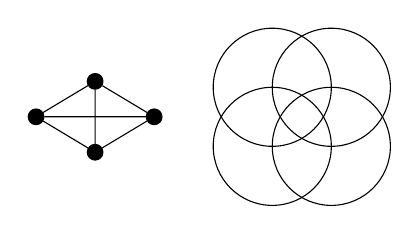
\begin{tikzpicture}[scale=1.5]

  \draw (-0.5,2.5) circle [radius=0.5];
  \draw (0,2.5) circle [radius=0.5];
  \draw (-0.5,2) circle [radius=0.5];
  \draw (0,2) circle [radius=0.5];


  \node[draw,circle,inner sep=2pt,fill,label distance=1cm] (v1) at (-2.5,2.25) {};

  \node[draw,circle,inner sep=2pt,fill,label distance=1cm] (v2) at (-2,1.95) {};
  \node[draw,circle,inner sep=2pt,fill,label distance=1cm] (v3) at (-2,2.55) {};
  \node[draw,circle,inner sep=2pt,fill,label distance=1cm] (v4) at (-1.5,2.25) {};

  \draw  (v3) edge (v2);
  \draw  (v4) edge (v1);
  \draw  (v3) edge (v1);
  \draw  (v4) edge (v2);
  \draw  (v3) edge (v4);
  \draw  (v1) edge (v2);

\end{tikzpicture}
\end{scaletikzpicturetowidth}

\caption{Realization of a UDG (unit disk graph).}
\label{fig:udg}
\end{figure}


An \emph{intersection graph} is a graph $G = (\zeta,E)$ of a collection of objects $\zeta$ is a graph such that $v,w \in \zeta$ and $v \cup w \neq \varnothing$ implies that $vw \in E$. An \emph{interval graph} is an intersection graph of intervals on the plane; when the size of the intervals is equal they are called \emph{unit interval graphs}. A \emph{unit disk graph} is an intersection graph of disks on a plane that have the same diameter - you can find an example in Figure \ref{fig:udg}.

\section{Order and set theory}

The \emph{powerset} $\powerset(S)$ of a set $S$ is the set of subsets of $S$. A \emph{partial order} is a binary relation $\leqslant$ over a set $A$ satisfying three axioms:

\begin{itemize}
  \item if $a \leqslant b$ and $b \leqslant a$ then $a = b$ (\emph{antisymmetry}).
  \item if $a \leqslant b$ and $b \leqslant c$ then $a \leqslant c$ (\emph{transitivity}).
  \item $a \leqslant a$ (\emph{reflexivity}).
\end{itemize}

\begin{figure}
\centering

\begin{scaletikzpicturetowidth}{\textwidth}
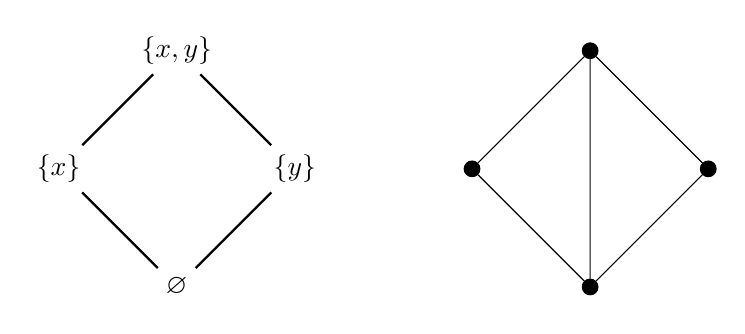
\begin{tikzpicture}[scale=1.5]

  % poset
  \draw (-1cm,0cm) node (v2) {$\{x\}$};
  \draw (1cm,0cm)  node (v3) { $\{y\}$ };
  \draw (0cm,-1cm) node (v4) {$\varnothing$};
  \draw (0cm,1cm)  node (v1) {$\{x,y\}$};

  \draw[thick]  (v1) edge (v2);
  \draw[thick]  (v3) edge (v1);
  \draw[thick]  (v3) edge (v4);
  \draw[thick]  (v2) edge (v4);

  % graph
  \node[draw,circle,inner sep=2pt,fill,label distance=1cm] (v1g) at (3.5,1) {};
  \node[draw,circle,inner sep=2pt,fill,label distance=1cm] (v2g) at (3.5,-1) {};
  \node[draw,circle,inner sep=2pt,fill,label distance=1cm] (v3g) at (4.5,0) {};
  \node[draw,circle,inner sep=2pt,fill,label distance=1cm] (v4g) at (2.5,0) {};
  \draw  (v1g) edge (v2g);
  \draw  (v1g) edge (v4g);
  \draw  (v4g) edge (v2g);
  \draw  (v1g) edge (v3g);
  \draw  (v3g) edge (v2g);

\end{tikzpicture}
\end{scaletikzpicturetowidth}

\caption{On the left, Hasse diagram of a poset of the power set of 2 elements ordered by inclusion.
On the right, the comparability graph of this poset.}
\label{fig:hasse}
\end{figure}

In the other side, a \emph{total order} is a partial order where the reflexivity order is replaced by the \emph{connexity} property -- $a \leq b\ \text{or}\  b \leq a$. A \emph{partially ordered set} (or \emph{poset}) $(S,\leqslant)$ is a set such that the elements of $S$ are partially ordered by the relation $\leqslant$. A good way to represent a poset is the \emph{Hasse diagram} (figure \ref{fig:hasse}).

\subsection{Comparability graphs}

A \emph{spanning order} $(V,<)$ on a graph $G = (V,E)$ is a total order on $V$ such that for any three vertices $u < v < w$:

  $$uw \in E \to uv \in E\ \text{or}\ vw \in E$$

The class of comparability graphs are built on the ideas of order theory. A graph $G$ is a \emph{comparability graph} if there exists a partial order $\leqslant$ such that $uv \in E \Leftrightarrow v \leqslant w\  \text{or}\  w \leqslant v$.

\section{Geometry}




\backmatter

\printindex % use makeindex to generate the index

\bibliographystyle{plain}

\bibliography{main} %use bibtex to generate the bibliography


\end{document}
